% Seminar 4: EVT, Copule și Managementul Riscului
% Statistica Piețelor Financiare

\documentclass[9pt, aspectratio=169, t]{beamer}
%=============================================================================
% PREAMBUL COMUN - Statistica Piețelor Financiare
% Prezentări academice de calitate Harvard
% Program de licență, Academia de Studii Economice din București
%
% Utilizare: \documentclass[9pt, aspectratio=169, t]{beamer}
%            %=============================================================================
% PREAMBUL COMUN - Statistica Piețelor Financiare
% Prezentări academice de calitate Harvard
% Program de licență, Academia de Studii Economice din București
%
% Utilizare: \documentclass[9pt, aspectratio=169, t]{beamer}
%            %=============================================================================
% PREAMBUL COMUN - Statistica Piețelor Financiare
% Prezentări academice de calitate Harvard
% Program de licență, Academia de Studii Economice din București
%
% Utilizare: \documentclass[9pt, aspectratio=169, t]{beamer}
%            \input{preamble}
%            \subtitle{Seminar X: Titlul Seminarului}
%            \begin{document} ...
%=============================================================================

% Asigură încadrarea conținutului pe diapozitive
\setbeamersize{text margin left=8mm, text margin right=8mm}

%=============================================================================
% CONFIGURARE TEMĂ ȘI STIL
%=============================================================================
\usetheme{default}

% Paletă de Culori
\definecolor{MainBlue}{RGB}{26, 58, 110}
\definecolor{AccentBlue}{RGB}{26, 58, 110}
\definecolor{IDAred}{RGB}{205, 0, 0}
\definecolor{DarkGray}{RGB}{51, 51, 51}
\definecolor{MediumGray}{RGB}{128, 128, 128}
\definecolor{LightGray}{RGB}{248, 248, 248}
\definecolor{VeryLightGray}{RGB}{235, 235, 235}
\definecolor{KeynoteGray}{RGB}{218, 218, 218}
\definecolor{SectionGray}{RGB}{120, 120, 120}
\definecolor{FooterGray}{RGB}{100, 100, 100}
\definecolor{Crimson}{RGB}{220, 53, 69}
\definecolor{Forest}{RGB}{46, 125, 50}
\definecolor{Amber}{RGB}{181, 133, 63}
\definecolor{Orange}{RGB}{230, 126, 34}
\definecolor{Purple}{RGB}{142, 68, 173}

% Fundal gradient (gradient Keynote exact 315°: alb la RGB 218,218,218)
\setbeamertemplate{background}{%
    \begin{tikzpicture}[remember picture, overlay]
        \shade[shading=axis, shading angle=315,
        top color=white, bottom color=KeynoteGray]
        (current page.south west) rectangle (current page.north east);
    \end{tikzpicture}%
}
% Culoare solidă de rezervă pentru compatibilitate
\setbeamercolor{background canvas}{bg=}

\setbeamercolor{palette primary}{bg=MainBlue, fg=white}
\setbeamercolor{palette secondary}{bg=MainBlue!85, fg=white}
\setbeamercolor{palette tertiary}{bg=MainBlue!70, fg=white}
\setbeamercolor{structure}{fg=MainBlue}
\setbeamercolor{title}{fg=IDAred}
\setbeamercolor{frametitle}{fg=IDAred, bg=}
\setbeamercolor{block title}{bg=MainBlue, fg=white}
\setbeamercolor{block body}{bg=VeryLightGray, fg=DarkGray}
\setbeamercolor{block title alerted}{bg=Crimson, fg=white}
\setbeamercolor{block body alerted}{bg=Crimson!8, fg=DarkGray}
\setbeamercolor{block title example}{bg=Forest, fg=white}
\setbeamercolor{block body example}{bg=Forest!8, fg=DarkGray}
\setbeamercolor{item}{fg=MainBlue}

% Font institute mai mic pentru a evita overfull hbox pe pagina de titlu
\setbeamerfont{institute}{size=\footnotesize}

% Culori subsol
\setbeamercolor{author in head/foot}{fg=FooterGray, bg=}
\setbeamercolor{title in head/foot}{fg=FooterGray, bg=}
\setbeamercolor{date in head/foot}{fg=FooterGray, bg=}
\setbeamercolor{section in head/foot}{fg=FooterGray, bg=}
\setbeamercolor{subsection in head/foot}{fg=FooterGray, bg=}

% Stiluri marcatori
\setbeamertemplate{itemize item}{\color{MainBlue}$\boxdot$}
\setbeamertemplate{itemize subitem}{\color{MainBlue}$\blacktriangleright$}
\setbeamertemplate{itemize subsubitem}{\color{MainBlue}\tiny$\bullet$}
\setbeamertemplate{itemize/enumerate body begin}{\normalsize}
\setbeamertemplate{itemize/enumerate subbody begin}{\normalsize}

% Stiluri cuprins (bullets în loc de numere)
\setbeamertemplate{section in toc}{%
    \leavevmode\leftskip=1.5em%
    \llap{\color{MainBlue}$\boxdot$\kern0.5em}%
    \inserttocsection\par%
}

% Spațiere compactă
\setlength{\leftmargini}{10pt}
\setlength{\leftmarginii}{10pt}
\makeatletter
\def\@listi{\leftmargin\leftmargini \topsep 0pt \parsep 0pt \itemsep 0pt}
\def\@listii{\leftmargin\leftmarginii \topsep 0pt \parsep 0pt \itemsep 0pt}
\makeatother

\setbeamertemplate{navigation symbols}{}

%=============================================================================
% ANTET PERSONALIZAT
%=============================================================================
\setbeamertemplate{headline}{%
    \vskip10pt%
    \hbox to \paperwidth{%
        \hskip0.5cm%
        {\small\color{FooterGray}\renewcommand{\hyperlink}[2]{##2}\insertsectionhead}%
        \hfill%
        \textcolor{FooterGray}{\small\insertframenumber}%
        \hskip0.5cm%
    }%
    \vskip4pt%
    {\color{FooterGray}\hrule height 0.4pt}%
}

%=============================================================================
% SUBSOL PERSONALIZAT
%=============================================================================
\usepackage{fontawesome5}

\setbeamertemplate{footline}{%
    {\color{FooterGray}\hrule height 0.4pt}%
    \vskip4pt%
    \hbox to \paperwidth{%
        \hskip0.5cm%
        \textcolor{FooterGray}{\small Statistica Piețelor Financiare}%
        \hfill%
        \raisebox{-0.1em}{%
            \begin{tikzpicture}[x=0.08em, y=0.08em, line width=0.4pt]
                \draw[FooterGray] (0,3) -- (1,4) -- (2,3.5) -- (3,5) -- (4,4) -- (5,6) -- (6,5.5) -- (7,4) -- (8,5) -- (9,7) -- (10,6) -- (11,5) -- (12,6.5) -- (13,8) -- (14,7) -- (15,6) -- (16,7.5) -- (17,9) -- (18,8) -- (19,7) -- (20,8.5) -- (21,10) -- (22,9) -- (23,8) -- (24,9.5);
            \end{tikzpicture}%
        }%
        \hskip0.5cm%
    }%
    \vskip6pt%
}

%=============================================================================
% PACHETE
%=============================================================================
\usepackage[utf8]{inputenc}
\usepackage[T1]{fontenc}
\usepackage{amsmath, amssymb, amsthm}
\usepackage{mathtools}
\usepackage{bm}
\usepackage{tikz}
\usetikzlibrary{arrows.meta, positioning, shapes, calc, decorations.pathreplacing, shadings}
\usepackage{booktabs}
\usepackage{multirow}
\usepackage{array}
\usepackage{graphicx}
\usepackage{hyperref}
\usepackage{colortbl}
\usepackage{listings}
\lstset{basicstyle=\ttfamily\small, breaklines=true, frame=single, backgroundcolor=\color{VeryLightGray}}
\hypersetup{colorlinks=true, linkcolor=MainBlue, urlcolor=MainBlue}
\graphicspath{{../../logos/}{../../charts/}{../../photos/}}
\hfuzz=2pt
\vfuzz=2pt

%=============================================================================
% COMANDA QUANTLET
%=============================================================================
\newcommand{\quantlet}[2]{%
    \hfill\href{#2}{%
        \raisebox{-0.15em}{
\includegraphics[height=0.7em]{ql_logo.png}}%
        \textcolor{MainBlue}{\tiny\ #1}%
    }%
}

%=============================================================================
% PAGINĂ TITLU PERSONALIZATĂ
%=============================================================================
\defbeamertemplate*{title page}{hybrid}[1][]
{
    \vspace{0.2cm}
    \begin{center}
        \href{https://www.ase.ro}{
\includegraphics[height=1.0cm]{ase_logo.png}}\hspace{0.25cm}%
        \href{https://theida.net}{
\includegraphics[height=1.0cm]{ida_logo.png}}\hspace{0.25cm}%
        \href{https://blockchain-research-center.com}{
\includegraphics[height=1.0cm]{brc_logo.png}}\hspace{0.25cm}%
        \href{https://www.ai4efin.ase.ro}{
\includegraphics[height=1.0cm]{ai4efin_logo.png}}\hspace{0.25cm}%
        \href{https://ipe.ro/new}{
\includegraphics[height=1.0cm]{acad_logo.png}}\hspace{0.25cm}%
        \href{https://www.digital-finance-msca.com}{
\includegraphics[height=1.0cm]{msca_logo.png}}%
    \end{center}

    \vspace{0.6cm}

    \begin{center}
        \begin{minipage}{0.1\textwidth}
            \centering
            \href{https://quantlet.com}{
\includegraphics[height=1.1cm]{ql_logo.png}}
        \end{minipage}%
        \begin{minipage}{0.78\textwidth}
            \centering
            {\LARGE\bfseries\usebeamercolor[fg]{title}\inserttitle}

            \vspace{0.3cm}

            {\usebeamerfont{subtitle}\usebeamercolor[fg]{title}\insertsubtitle}
        \end{minipage}%
        \begin{minipage}{0.1\textwidth}
            \centering
            \href{https://quantinar.com}{
\includegraphics[height=1.1cm]{qr_logo.png}}
        \end{minipage}
    \end{center}

    \vspace{0.6cm}

    \hspace{0.5cm}{\usebeamerfont{author}\insertauthor}

    \vspace{0.3cm}

    \hspace{0.5cm}\begin{minipage}[t]{0.9\textwidth}
        \raggedright\small\insertinstitute
    \end{minipage}
}

%=============================================================================
% MEDII PENTRU TEOREME
%=============================================================================
\theoremstyle{definition}
\setbeamertemplate{theorems}[numbered]
\newtheorem{defn}{Definiție}
\newtheorem{thm}{Teoremă}
\newtheorem{prop}{Propoziție}
\newtheorem{rmk}{Observație}

%=============================================================================
% CENTRED MINIPAGE
%=============================================================================
\newenvironment{cminipage}[1]{%
    \par\noindent\hfill\begin{minipage}{#1}\ignorespaces
}{%
    \end{minipage}\hfill\null\par
}

%=============================================================================
% COMENZI PERSONALIZATE
%=============================================================================
\newcommand{\E}{\mathbb{E}}
\newcommand{\Var}{\text{Var}}
\newcommand{\Cov}{\text{Cov}}
\newcommand{\Corr}{\text{Corr}}
\newcommand{\R}{\mathbb{R}}
\newcommand{\N}{\mathbb{N}}
\newcommand{\Z}{\mathbb{Z}}
\newcommand{\B}{\mathbf{B}}
\newcommand{\imark}{\textcolor{MainBlue}{\textbullet}}
\newcommand{\RMSE}{\text{RMSE}}
\newcommand{\MAE}{\text{MAE}}
\newcommand{\MAPE}{\text{MAPE}}
\newcommand{\correct}{\textcolor{Forest}{\checkmark}}
\newcommand{\incorrect}{\textcolor{Crimson}{\texttimes}}

%=============================================================================
% INFORMAȚII TITLU
%=============================================================================
\title[Statistica Piețelor Financiare]{Statistica Piețelor Financiare}
\author[D.T. Pele, A. Amza]{\texorpdfstring{\begin{tabular}[t]{@{}l@{}}Daniel Traian PELE \\ Antoaneta Amza\end{tabular}}{Daniel Traian PELE, Antoaneta Amza}}
\institute{Academia de Studii Economice din București\\
IDA Institute Digital Assets\\
Blockchain Research Center\\
AI4EFin Artificial Intelligence for Energy Finance\\
Academia Română, Institutul de Prognoză Economică\\
MSCA Digital Finance}
\date{}

%            \subtitle{Seminar X: Titlul Seminarului}
%            \begin{document} ...
%=============================================================================

% Asigură încadrarea conținutului pe diapozitive
\setbeamersize{text margin left=8mm, text margin right=8mm}

%=============================================================================
% CONFIGURARE TEMĂ ȘI STIL
%=============================================================================
\usetheme{default}

% Paletă de Culori
\definecolor{MainBlue}{RGB}{26, 58, 110}
\definecolor{AccentBlue}{RGB}{26, 58, 110}
\definecolor{IDAred}{RGB}{205, 0, 0}
\definecolor{DarkGray}{RGB}{51, 51, 51}
\definecolor{MediumGray}{RGB}{128, 128, 128}
\definecolor{LightGray}{RGB}{248, 248, 248}
\definecolor{VeryLightGray}{RGB}{235, 235, 235}
\definecolor{KeynoteGray}{RGB}{218, 218, 218}
\definecolor{SectionGray}{RGB}{120, 120, 120}
\definecolor{FooterGray}{RGB}{100, 100, 100}
\definecolor{Crimson}{RGB}{220, 53, 69}
\definecolor{Forest}{RGB}{46, 125, 50}
\definecolor{Amber}{RGB}{181, 133, 63}
\definecolor{Orange}{RGB}{230, 126, 34}
\definecolor{Purple}{RGB}{142, 68, 173}

% Fundal gradient (gradient Keynote exact 315°: alb la RGB 218,218,218)
\setbeamertemplate{background}{%
    \begin{tikzpicture}[remember picture, overlay]
        \shade[shading=axis, shading angle=315,
        top color=white, bottom color=KeynoteGray]
        (current page.south west) rectangle (current page.north east);
    \end{tikzpicture}%
}
% Culoare solidă de rezervă pentru compatibilitate
\setbeamercolor{background canvas}{bg=}

\setbeamercolor{palette primary}{bg=MainBlue, fg=white}
\setbeamercolor{palette secondary}{bg=MainBlue!85, fg=white}
\setbeamercolor{palette tertiary}{bg=MainBlue!70, fg=white}
\setbeamercolor{structure}{fg=MainBlue}
\setbeamercolor{title}{fg=IDAred}
\setbeamercolor{frametitle}{fg=IDAred, bg=}
\setbeamercolor{block title}{bg=MainBlue, fg=white}
\setbeamercolor{block body}{bg=VeryLightGray, fg=DarkGray}
\setbeamercolor{block title alerted}{bg=Crimson, fg=white}
\setbeamercolor{block body alerted}{bg=Crimson!8, fg=DarkGray}
\setbeamercolor{block title example}{bg=Forest, fg=white}
\setbeamercolor{block body example}{bg=Forest!8, fg=DarkGray}
\setbeamercolor{item}{fg=MainBlue}

% Font institute mai mic pentru a evita overfull hbox pe pagina de titlu
\setbeamerfont{institute}{size=\footnotesize}

% Culori subsol
\setbeamercolor{author in head/foot}{fg=FooterGray, bg=}
\setbeamercolor{title in head/foot}{fg=FooterGray, bg=}
\setbeamercolor{date in head/foot}{fg=FooterGray, bg=}
\setbeamercolor{section in head/foot}{fg=FooterGray, bg=}
\setbeamercolor{subsection in head/foot}{fg=FooterGray, bg=}

% Stiluri marcatori
\setbeamertemplate{itemize item}{\color{MainBlue}$\boxdot$}
\setbeamertemplate{itemize subitem}{\color{MainBlue}$\blacktriangleright$}
\setbeamertemplate{itemize subsubitem}{\color{MainBlue}\tiny$\bullet$}
\setbeamertemplate{itemize/enumerate body begin}{\normalsize}
\setbeamertemplate{itemize/enumerate subbody begin}{\normalsize}

% Stiluri cuprins (bullets în loc de numere)
\setbeamertemplate{section in toc}{%
    \leavevmode\leftskip=1.5em%
    \llap{\color{MainBlue}$\boxdot$\kern0.5em}%
    \inserttocsection\par%
}

% Spațiere compactă
\setlength{\leftmargini}{10pt}
\setlength{\leftmarginii}{10pt}
\makeatletter
\def\@listi{\leftmargin\leftmargini \topsep 0pt \parsep 0pt \itemsep 0pt}
\def\@listii{\leftmargin\leftmarginii \topsep 0pt \parsep 0pt \itemsep 0pt}
\makeatother

\setbeamertemplate{navigation symbols}{}

%=============================================================================
% ANTET PERSONALIZAT
%=============================================================================
\setbeamertemplate{headline}{%
    \vskip10pt%
    \hbox to \paperwidth{%
        \hskip0.5cm%
        {\small\color{FooterGray}\renewcommand{\hyperlink}[2]{##2}\insertsectionhead}%
        \hfill%
        \textcolor{FooterGray}{\small\insertframenumber}%
        \hskip0.5cm%
    }%
    \vskip4pt%
    {\color{FooterGray}\hrule height 0.4pt}%
}

%=============================================================================
% SUBSOL PERSONALIZAT
%=============================================================================
\usepackage{fontawesome5}

\setbeamertemplate{footline}{%
    {\color{FooterGray}\hrule height 0.4pt}%
    \vskip4pt%
    \hbox to \paperwidth{%
        \hskip0.5cm%
        \textcolor{FooterGray}{\small Statistica Piețelor Financiare}%
        \hfill%
        \raisebox{-0.1em}{%
            \begin{tikzpicture}[x=0.08em, y=0.08em, line width=0.4pt]
                \draw[FooterGray] (0,3) -- (1,4) -- (2,3.5) -- (3,5) -- (4,4) -- (5,6) -- (6,5.5) -- (7,4) -- (8,5) -- (9,7) -- (10,6) -- (11,5) -- (12,6.5) -- (13,8) -- (14,7) -- (15,6) -- (16,7.5) -- (17,9) -- (18,8) -- (19,7) -- (20,8.5) -- (21,10) -- (22,9) -- (23,8) -- (24,9.5);
            \end{tikzpicture}%
        }%
        \hskip0.5cm%
    }%
    \vskip6pt%
}

%=============================================================================
% PACHETE
%=============================================================================
\usepackage[utf8]{inputenc}
\usepackage[T1]{fontenc}
\usepackage{amsmath, amssymb, amsthm}
\usepackage{mathtools}
\usepackage{bm}
\usepackage{tikz}
\usetikzlibrary{arrows.meta, positioning, shapes, calc, decorations.pathreplacing, shadings}
\usepackage{booktabs}
\usepackage{multirow}
\usepackage{array}
\usepackage{graphicx}
\usepackage{hyperref}
\usepackage{colortbl}
\usepackage{listings}
\lstset{basicstyle=\ttfamily\small, breaklines=true, frame=single, backgroundcolor=\color{VeryLightGray}}
\hypersetup{colorlinks=true, linkcolor=MainBlue, urlcolor=MainBlue}
\graphicspath{{../../logos/}{../../charts/}{../../photos/}}
\hfuzz=2pt
\vfuzz=2pt

%=============================================================================
% COMANDA QUANTLET
%=============================================================================
\newcommand{\quantlet}[2]{%
    \hfill\href{#2}{%
        \raisebox{-0.15em}{
\includegraphics[height=0.7em]{ql_logo.png}}%
        \textcolor{MainBlue}{\tiny\ #1}%
    }%
}

%=============================================================================
% PAGINĂ TITLU PERSONALIZATĂ
%=============================================================================
\defbeamertemplate*{title page}{hybrid}[1][]
{
    \vspace{0.2cm}
    \begin{center}
        \href{https://www.ase.ro}{
\includegraphics[height=1.0cm]{ase_logo.png}}\hspace{0.25cm}%
        \href{https://theida.net}{
\includegraphics[height=1.0cm]{ida_logo.png}}\hspace{0.25cm}%
        \href{https://blockchain-research-center.com}{
\includegraphics[height=1.0cm]{brc_logo.png}}\hspace{0.25cm}%
        \href{https://www.ai4efin.ase.ro}{
\includegraphics[height=1.0cm]{ai4efin_logo.png}}\hspace{0.25cm}%
        \href{https://ipe.ro/new}{
\includegraphics[height=1.0cm]{acad_logo.png}}\hspace{0.25cm}%
        \href{https://www.digital-finance-msca.com}{
\includegraphics[height=1.0cm]{msca_logo.png}}%
    \end{center}

    \vspace{0.6cm}

    \begin{center}
        \begin{minipage}{0.1\textwidth}
            \centering
            \href{https://quantlet.com}{
\includegraphics[height=1.1cm]{ql_logo.png}}
        \end{minipage}%
        \begin{minipage}{0.78\textwidth}
            \centering
            {\LARGE\bfseries\usebeamercolor[fg]{title}\inserttitle}

            \vspace{0.3cm}

            {\usebeamerfont{subtitle}\usebeamercolor[fg]{title}\insertsubtitle}
        \end{minipage}%
        \begin{minipage}{0.1\textwidth}
            \centering
            \href{https://quantinar.com}{
\includegraphics[height=1.1cm]{qr_logo.png}}
        \end{minipage}
    \end{center}

    \vspace{0.6cm}

    \hspace{0.5cm}{\usebeamerfont{author}\insertauthor}

    \vspace{0.3cm}

    \hspace{0.5cm}\begin{minipage}[t]{0.9\textwidth}
        \raggedright\small\insertinstitute
    \end{minipage}
}

%=============================================================================
% MEDII PENTRU TEOREME
%=============================================================================
\theoremstyle{definition}
\setbeamertemplate{theorems}[numbered]
\newtheorem{defn}{Definiție}
\newtheorem{thm}{Teoremă}
\newtheorem{prop}{Propoziție}
\newtheorem{rmk}{Observație}

%=============================================================================
% CENTRED MINIPAGE
%=============================================================================
\newenvironment{cminipage}[1]{%
    \par\noindent\hfill\begin{minipage}{#1}\ignorespaces
}{%
    \end{minipage}\hfill\null\par
}

%=============================================================================
% COMENZI PERSONALIZATE
%=============================================================================
\newcommand{\E}{\mathbb{E}}
\newcommand{\Var}{\text{Var}}
\newcommand{\Cov}{\text{Cov}}
\newcommand{\Corr}{\text{Corr}}
\newcommand{\R}{\mathbb{R}}
\newcommand{\N}{\mathbb{N}}
\newcommand{\Z}{\mathbb{Z}}
\newcommand{\B}{\mathbf{B}}
\newcommand{\imark}{\textcolor{MainBlue}{\textbullet}}
\newcommand{\RMSE}{\text{RMSE}}
\newcommand{\MAE}{\text{MAE}}
\newcommand{\MAPE}{\text{MAPE}}
\newcommand{\correct}{\textcolor{Forest}{\checkmark}}
\newcommand{\incorrect}{\textcolor{Crimson}{\texttimes}}

%=============================================================================
% INFORMAȚII TITLU
%=============================================================================
\title[Statistica Piețelor Financiare]{Statistica Piețelor Financiare}
\author[D.T. Pele, A. Amza]{\texorpdfstring{\begin{tabular}[t]{@{}l@{}}Daniel Traian PELE \\ Antoaneta Amza\end{tabular}}{Daniel Traian PELE, Antoaneta Amza}}
\institute{Academia de Studii Economice din București\\
IDA Institute Digital Assets\\
Blockchain Research Center\\
AI4EFin Artificial Intelligence for Energy Finance\\
Academia Română, Institutul de Prognoză Economică\\
MSCA Digital Finance}
\date{}

%            \subtitle{Seminar X: Titlul Seminarului}
%            \begin{document} ...
%=============================================================================

% Asigură încadrarea conținutului pe diapozitive
\setbeamersize{text margin left=8mm, text margin right=8mm}

%=============================================================================
% CONFIGURARE TEMĂ ȘI STIL
%=============================================================================
\usetheme{default}

% Paletă de Culori
\definecolor{MainBlue}{RGB}{26, 58, 110}
\definecolor{AccentBlue}{RGB}{26, 58, 110}
\definecolor{IDAred}{RGB}{205, 0, 0}
\definecolor{DarkGray}{RGB}{51, 51, 51}
\definecolor{MediumGray}{RGB}{128, 128, 128}
\definecolor{LightGray}{RGB}{248, 248, 248}
\definecolor{VeryLightGray}{RGB}{235, 235, 235}
\definecolor{KeynoteGray}{RGB}{218, 218, 218}
\definecolor{SectionGray}{RGB}{120, 120, 120}
\definecolor{FooterGray}{RGB}{100, 100, 100}
\definecolor{Crimson}{RGB}{220, 53, 69}
\definecolor{Forest}{RGB}{46, 125, 50}
\definecolor{Amber}{RGB}{181, 133, 63}
\definecolor{Orange}{RGB}{230, 126, 34}
\definecolor{Purple}{RGB}{142, 68, 173}

% Fundal gradient (gradient Keynote exact 315°: alb la RGB 218,218,218)
\setbeamertemplate{background}{%
    \begin{tikzpicture}[remember picture, overlay]
        \shade[shading=axis, shading angle=315,
        top color=white, bottom color=KeynoteGray]
        (current page.south west) rectangle (current page.north east);
    \end{tikzpicture}%
}
% Culoare solidă de rezervă pentru compatibilitate
\setbeamercolor{background canvas}{bg=}

\setbeamercolor{palette primary}{bg=MainBlue, fg=white}
\setbeamercolor{palette secondary}{bg=MainBlue!85, fg=white}
\setbeamercolor{palette tertiary}{bg=MainBlue!70, fg=white}
\setbeamercolor{structure}{fg=MainBlue}
\setbeamercolor{title}{fg=IDAred}
\setbeamercolor{frametitle}{fg=IDAred, bg=}
\setbeamercolor{block title}{bg=MainBlue, fg=white}
\setbeamercolor{block body}{bg=VeryLightGray, fg=DarkGray}
\setbeamercolor{block title alerted}{bg=Crimson, fg=white}
\setbeamercolor{block body alerted}{bg=Crimson!8, fg=DarkGray}
\setbeamercolor{block title example}{bg=Forest, fg=white}
\setbeamercolor{block body example}{bg=Forest!8, fg=DarkGray}
\setbeamercolor{item}{fg=MainBlue}

% Font institute mai mic pentru a evita overfull hbox pe pagina de titlu
\setbeamerfont{institute}{size=\footnotesize}

% Culori subsol
\setbeamercolor{author in head/foot}{fg=FooterGray, bg=}
\setbeamercolor{title in head/foot}{fg=FooterGray, bg=}
\setbeamercolor{date in head/foot}{fg=FooterGray, bg=}
\setbeamercolor{section in head/foot}{fg=FooterGray, bg=}
\setbeamercolor{subsection in head/foot}{fg=FooterGray, bg=}

% Stiluri marcatori
\setbeamertemplate{itemize item}{\color{MainBlue}$\boxdot$}
\setbeamertemplate{itemize subitem}{\color{MainBlue}$\blacktriangleright$}
\setbeamertemplate{itemize subsubitem}{\color{MainBlue}\tiny$\bullet$}
\setbeamertemplate{itemize/enumerate body begin}{\normalsize}
\setbeamertemplate{itemize/enumerate subbody begin}{\normalsize}

% Stiluri cuprins (bullets în loc de numere)
\setbeamertemplate{section in toc}{%
    \leavevmode\leftskip=1.5em%
    \llap{\color{MainBlue}$\boxdot$\kern0.5em}%
    \inserttocsection\par%
}

% Spațiere compactă
\setlength{\leftmargini}{10pt}
\setlength{\leftmarginii}{10pt}
\makeatletter
\def\@listi{\leftmargin\leftmargini \topsep 0pt \parsep 0pt \itemsep 0pt}
\def\@listii{\leftmargin\leftmarginii \topsep 0pt \parsep 0pt \itemsep 0pt}
\makeatother

\setbeamertemplate{navigation symbols}{}

%=============================================================================
% ANTET PERSONALIZAT
%=============================================================================
\setbeamertemplate{headline}{%
    \vskip10pt%
    \hbox to \paperwidth{%
        \hskip0.5cm%
        {\small\color{FooterGray}\renewcommand{\hyperlink}[2]{##2}\insertsectionhead}%
        \hfill%
        \textcolor{FooterGray}{\small\insertframenumber}%
        \hskip0.5cm%
    }%
    \vskip4pt%
    {\color{FooterGray}\hrule height 0.4pt}%
}

%=============================================================================
% SUBSOL PERSONALIZAT
%=============================================================================
\usepackage{fontawesome5}

\setbeamertemplate{footline}{%
    {\color{FooterGray}\hrule height 0.4pt}%
    \vskip4pt%
    \hbox to \paperwidth{%
        \hskip0.5cm%
        \textcolor{FooterGray}{\small Statistica Piețelor Financiare}%
        \hfill%
        \raisebox{-0.1em}{%
            \begin{tikzpicture}[x=0.08em, y=0.08em, line width=0.4pt]
                \draw[FooterGray] (0,3) -- (1,4) -- (2,3.5) -- (3,5) -- (4,4) -- (5,6) -- (6,5.5) -- (7,4) -- (8,5) -- (9,7) -- (10,6) -- (11,5) -- (12,6.5) -- (13,8) -- (14,7) -- (15,6) -- (16,7.5) -- (17,9) -- (18,8) -- (19,7) -- (20,8.5) -- (21,10) -- (22,9) -- (23,8) -- (24,9.5);
            \end{tikzpicture}%
        }%
        \hskip0.5cm%
    }%
    \vskip6pt%
}

%=============================================================================
% PACHETE
%=============================================================================
\usepackage[utf8]{inputenc}
\usepackage[T1]{fontenc}
\usepackage{amsmath, amssymb, amsthm}
\usepackage{mathtools}
\usepackage{bm}
\usepackage{tikz}
\usetikzlibrary{arrows.meta, positioning, shapes, calc, decorations.pathreplacing, shadings}
\usepackage{booktabs}
\usepackage{multirow}
\usepackage{array}
\usepackage{graphicx}
\usepackage{hyperref}
\usepackage{colortbl}
\usepackage{listings}
\lstset{basicstyle=\ttfamily\small, breaklines=true, frame=single, backgroundcolor=\color{VeryLightGray}}
\hypersetup{colorlinks=true, linkcolor=MainBlue, urlcolor=MainBlue}
\graphicspath{{../../logos/}{../../charts/}{../../photos/}}
\hfuzz=2pt
\vfuzz=2pt

%=============================================================================
% COMANDA QUANTLET
%=============================================================================
\newcommand{\quantlet}[2]{%
    \hfill\href{#2}{%
        \raisebox{-0.15em}{
\includegraphics[height=0.7em]{ql_logo.png}}%
        \textcolor{MainBlue}{\tiny\ #1}%
    }%
}

%=============================================================================
% PAGINĂ TITLU PERSONALIZATĂ
%=============================================================================
\defbeamertemplate*{title page}{hybrid}[1][]
{
    \vspace{0.2cm}
    \begin{center}
        \href{https://www.ase.ro}{
\includegraphics[height=1.0cm]{ase_logo.png}}\hspace{0.25cm}%
        \href{https://theida.net}{
\includegraphics[height=1.0cm]{ida_logo.png}}\hspace{0.25cm}%
        \href{https://blockchain-research-center.com}{
\includegraphics[height=1.0cm]{brc_logo.png}}\hspace{0.25cm}%
        \href{https://www.ai4efin.ase.ro}{
\includegraphics[height=1.0cm]{ai4efin_logo.png}}\hspace{0.25cm}%
        \href{https://ipe.ro/new}{
\includegraphics[height=1.0cm]{acad_logo.png}}\hspace{0.25cm}%
        \href{https://www.digital-finance-msca.com}{
\includegraphics[height=1.0cm]{msca_logo.png}}%
    \end{center}

    \vspace{0.6cm}

    \begin{center}
        \begin{minipage}{0.1\textwidth}
            \centering
            \href{https://quantlet.com}{
\includegraphics[height=1.1cm]{ql_logo.png}}
        \end{minipage}%
        \begin{minipage}{0.78\textwidth}
            \centering
            {\LARGE\bfseries\usebeamercolor[fg]{title}\inserttitle}

            \vspace{0.3cm}

            {\usebeamerfont{subtitle}\usebeamercolor[fg]{title}\insertsubtitle}
        \end{minipage}%
        \begin{minipage}{0.1\textwidth}
            \centering
            \href{https://quantinar.com}{
\includegraphics[height=1.1cm]{qr_logo.png}}
        \end{minipage}
    \end{center}

    \vspace{0.6cm}

    \hspace{0.5cm}{\usebeamerfont{author}\insertauthor}

    \vspace{0.3cm}

    \hspace{0.5cm}\begin{minipage}[t]{0.9\textwidth}
        \raggedright\small\insertinstitute
    \end{minipage}
}

%=============================================================================
% MEDII PENTRU TEOREME
%=============================================================================
\theoremstyle{definition}
\setbeamertemplate{theorems}[numbered]
\newtheorem{defn}{Definiție}
\newtheorem{thm}{Teoremă}
\newtheorem{prop}{Propoziție}
\newtheorem{rmk}{Observație}

%=============================================================================
% CENTRED MINIPAGE
%=============================================================================
\newenvironment{cminipage}[1]{%
    \par\noindent\hfill\begin{minipage}{#1}\ignorespaces
}{%
    \end{minipage}\hfill\null\par
}

%=============================================================================
% COMENZI PERSONALIZATE
%=============================================================================
\newcommand{\E}{\mathbb{E}}
\newcommand{\Var}{\text{Var}}
\newcommand{\Cov}{\text{Cov}}
\newcommand{\Corr}{\text{Corr}}
\newcommand{\R}{\mathbb{R}}
\newcommand{\N}{\mathbb{N}}
\newcommand{\Z}{\mathbb{Z}}
\newcommand{\B}{\mathbf{B}}
\newcommand{\imark}{\textcolor{MainBlue}{\textbullet}}
\newcommand{\RMSE}{\text{RMSE}}
\newcommand{\MAE}{\text{MAE}}
\newcommand{\MAPE}{\text{MAPE}}
\newcommand{\correct}{\textcolor{Forest}{\checkmark}}
\newcommand{\incorrect}{\textcolor{Crimson}{\texttimes}}

%=============================================================================
% INFORMAȚII TITLU
%=============================================================================
\title[Statistica Piețelor Financiare]{Statistica Piețelor Financiare}
\author[D.T. Pele, A. Amza]{\texorpdfstring{\begin{tabular}[t]{@{}l@{}}Daniel Traian PELE \\ Antoaneta Amza\end{tabular}}{Daniel Traian PELE, Antoaneta Amza}}
\institute{Academia de Studii Economice din București\\
IDA Institute Digital Assets\\
Blockchain Research Center\\
AI4EFin Artificial Intelligence for Energy Finance\\
Academia Română, Institutul de Prognoză Economică\\
MSCA Digital Finance}
\date{}

\subtitle{Seminar 4: EVT, Copule și Managementul Riscului}

\begin{document}

%=============================================================================
% PAGINA DE TITLU
%=============================================================================
{
\setbeamertemplate{headline}{}
\setbeamertemplate{footline}{}
\begin{frame}
    \titlepage
\end{frame}
}

%=============================================================================
% CUPRINS SEMINAR
%=============================================================================
\begin{frame}{Cuprins Seminar}
    \begin{cminipage}{0.95\textwidth}
    \begin{itemize}\setlength{\itemsep}{0pt}
        \item \textbf{Obiective} -- Competențe vizate, recapitulare formule cheie
        \vspace{0.1cm}
        \item \textbf{Partea I: EVT manual} -- GEV, GPD, POT, estimatorul Hill, Mean Excess
        \vspace{0.1cm}
        \item \textbf{Partea II: Compararea distribuțiilor} -- AIC, BIC, QQ-plot, backtesting VaR
        \vspace{0.1cm}
        \item \textbf{Partea III: Copule} -- Gaussiană, Student-$t$, Clayton, Gumbel, dependența de coadă
        \vspace{0.1cm}
        \item \textbf{Partea IV: Managementul riscului} -- VaR, ES, subaditivitate, Kupiec, Basel~III
        \vspace{0.1cm}
        \item \textbf{Partea V: Python} -- EVT fit, backtesting, copule, GARCH
        \vspace{0.1cm}
        \item \textbf{Discuții și AI} -- Scenarii practice, verificarea codului AI
        \vspace{0.1cm}
        \item \textbf{Test rapid} -- 8 întrebări cu răspunsuri detaliate
        \vspace{0.1cm}
        \item \textbf{Rezumat și Bibliografie} -- Checklist, referințe, tema pentru acasă
    \end{itemize}
    \end{cminipage}
\end{frame}

%=============================================================================
% OBIECTIVE
%=============================================================================
\section{Obiective}

\begin{frame}{Obiective de învățare}
    \begin{cminipage}{0.95\textwidth}
\begin{columns}[T]
\begin{column}{0.55\textwidth}
\begin{block}{La finalul seminarului veți putea:}
\begin{itemize}\setlength{\itemsep}{0pt}
    \item Aplica metoda POT: alege pragul $u$, ajusta GPD, calcula VaR/ES
    \item Utiliza estimatorul Hill pentru indicele de coadă
    \item Compara distribuții prin AIC, BIC, teste KS și grafice QQ
    \item Descrie copulele principale și dependența de coadă
    \item Calcula VaR și ES sub diferite ipoteze distribuționale
    \item Efectua backtesting VaR cu testul Kupiec
\end{itemize}
\end{block}
\end{column}
\begin{column}{0.42\textwidth}
\begin{center}
\begin{tikzpicture}[
    node distance=0.35cm,
    every node/.style={font=\scriptsize, align=center},
    phase/.style={draw=MainBlue, fill=MainBlue!8, rounded corners=3pt,
                  minimum width=3.8cm, minimum height=0.55cm}
]
\node[phase] (p1) {I. EVT manual (25 min)};
\node[phase, below=of p1] (p2) {II. Comparare (15 min)};
\node[phase, below=of p2] (p3) {III. Copule (15 min)};
\node[phase, below=of p3] (p4) {IV. Risc (15 min)};
\node[phase, below=of p4] (p5) {V. Python (20 min)};
\draw[-{Stealth}, MainBlue, thick] (p1) -- (p2);
\draw[-{Stealth}, MainBlue, thick] (p2) -- (p3);
\draw[-{Stealth}, MainBlue, thick] (p3) -- (p4);
\draw[-{Stealth}, MainBlue, thick] (p4) -- (p5);
\end{tikzpicture}
\end{center}
\end{column}
\end{columns}
    \end{cminipage}
\end{frame}

\begin{frame}{Recapitulare: Formule cheie din curs}
\begin{cminipage}{0.95\textwidth}
\begin{columns}[T]
\begin{column}{0.48\textwidth}
\begin{block}{EVT --- Extreme Value Theory}
\begin{itemize}\setlength{\itemsep}{0pt}
    \item \textbf{GEV:} $H_\xi(x) = \exp\{-(1+\xi x)^{-1/\xi}\}$
    \item \textbf{GPD:} $G_{\xi,\sigma}(y) = 1 - (1+\xi y/\sigma)^{-1/\xi}$
    \item \textbf{VaR POT:}
    $$\text{VaR}_\alpha = u + \frac{\hat{\sigma}}{\hat{\xi}}\left[\left(\frac{n}{N_u}\alpha\right)^{-\hat{\xi}} - 1\right]$$
    \item \textbf{ES POT:}
    $$\text{ES}_\alpha = \frac{\text{VaR}_\alpha}{1-\hat{\xi}} + \frac{\hat{\sigma} - \hat{\xi}u}{1-\hat{\xi}}$$
\end{itemize}
\end{block}
\end{column}
\begin{column}{0.48\textwidth}
\begin{block}{Selecția modelului}
\begin{itemize}\setlength{\itemsep}{0pt}
    \item \textbf{AIC:} $-2\ell + 2k$
    \item \textbf{BIC:} $-2\ell + k\ln n$
    \item \textbf{Hill:} $\hat{\alpha}_H = \left[\frac{1}{k}\sum_{i=1}^k \ln\frac{X_{(i)}}{X_{(k+1)}}\right]^{-1}$
\end{itemize}
\end{block}
\begin{alertblock}{Măsuri de risc}
\begin{itemize}\setlength{\itemsep}{0pt}
    \item \textbf{VaR:} $P(X \leq -\text{VaR}_\alpha) = \alpha$
    \item \textbf{ES:} $\E[-X \mid X \leq -\text{VaR}_\alpha]$
    \item \textbf{Kupiec:} $LR \sim \chi^2(1)$
\end{itemize}
\end{alertblock}
\end{column}
\end{columns}
\end{cminipage}
\end{frame}

%=============================================================================
% PARTEA I: EVT MANUAL
%=============================================================================
\section{Partea I: EVT manual}

\begin{frame}{Exercițiul 1: Parametrul de formă GEV --- Interpretare}
    \begin{cminipage}{0.95\textwidth}
\begin{block}{Problemă}
\begin{itemize}\setlength{\itemsep}{0pt}
    \item Maximele lunare ale pierderilor zilnice pe S\&P~500 (20 ani, $n=240$ blocuri) sunt ajustate cu GEV. Rezultat: $\hat{\xi} = 0{,}28$, $\hat{\mu} = 1{,}8\%$, $\hat{\sigma} = 0{,}9\%$.
    \item (a) Ce tip de GEV este? (b) Ce implică $\xi > 0$ pentru cozi? (c) Calculați cuantila 99\%.
\end{itemize}
\end{block}

\begin{exampleblock}{Rezolvare}
\begin{itemize}\setlength{\itemsep}{0pt}
    \item (a) $\xi > 0$ $\Rightarrow$ \textbf{Fréchet} (cozi groase, lege putere). Celelalte: Gumbel ($\xi = 0$), Weibull ($\xi < 0$).
    \item (b) Coada superioară scade ca $x^{-1/\xi} = x^{-3{,}57}$. Momente de ordin $\geq 1/\xi \approx 3{,}6$ nu există.
    \item (c) Cuantila 99\%: $x_{0{,}99} = \hat{\mu} + \frac{\hat{\sigma}}{\hat{\xi}}\left[(-\ln 0{,}99)^{-\hat{\xi}} - 1\right]$
    $= 1{,}8\% + \frac{0{,}9\%}{0{,}28}\left[(0{,}01005)^{-0{,}28} - 1\right] = 1{,}8\% + 3{,}214\% \times (3{,}72 - 1) = \mathbf{10{,}5\%}$
\end{itemize}
\end{exampleblock}
    \end{cminipage}
\end{frame}

\begin{frame}{Exercițiul 2: Metoda POT --- Pas cu pas}
    \begin{cminipage}{0.95\textwidth}
\begin{block}{Problemă}
\begin{itemize}\setlength{\itemsep}{0pt}
    \item Din $n = 1{.}000$ randamente zilnice, $N_u = 50$ depășesc pragul $u = 2{,}5\%$ (în valoare absolută). GPD ajustată pe excese: $\hat{\xi} = 0{,}3$, $\hat{\sigma} = 0{,}8\%$. Calculați VaR și ES la 1\%.
\end{itemize}
\end{block}

\begin{exampleblock}{Rezolvare}
\begin{enumerate}\setlength{\itemsep}{0pt}
    \item Raportul: $\frac{n\alpha}{N_u} = \frac{1000 \times 0{,}01}{50} = 0{,}2$; \quad $0{,}2^{-0{,}3} = 1{,}621$
    \item $\text{VaR}_{1\%} = u + \frac{\hat{\sigma}}{\hat{\xi}}[0{,}2^{-\hat{\xi}} - 1] = 2{,}5\% + \frac{0{,}8\%}{0{,}3} \times 0{,}621 = 2{,}5\% + 1{,}66\% = \mathbf{4{,}16\%}$
    \item $\text{ES}_{1\%} = \frac{\text{VaR}}{1-\hat{\xi}} + \frac{\hat{\sigma} - \hat{\xi}u}{1-\hat{\xi}} = \frac{4{,}16\%}{0{,}7} + \frac{0{,}8\% - 0{,}75\%}{0{,}7} = 5{,}94\% + 0{,}07\% = \mathbf{6{,}01\%}$
    \item \textbf{Interpretare:} Pierderea medie \textit{dincolo} de VaR este 6{,}01\%, cu 44\% mai mare decât VaR!
\end{enumerate}
\end{exampleblock}
    \end{cminipage}
\end{frame}

\begin{frame}{Graficul Mean Excess --- Alegerea pragului $u$}
    \begin{cminipage}{0.95\textwidth}
\quantlet{SFM\_ch2\_extreme\_value}{https://github.com/QuantLet/Stat_fin_markets/tree/master/Ch_02/SFM_ch2_extreme_value}

\begin{columns}[T]
\begin{column}{0.45\textwidth}
\begin{center}
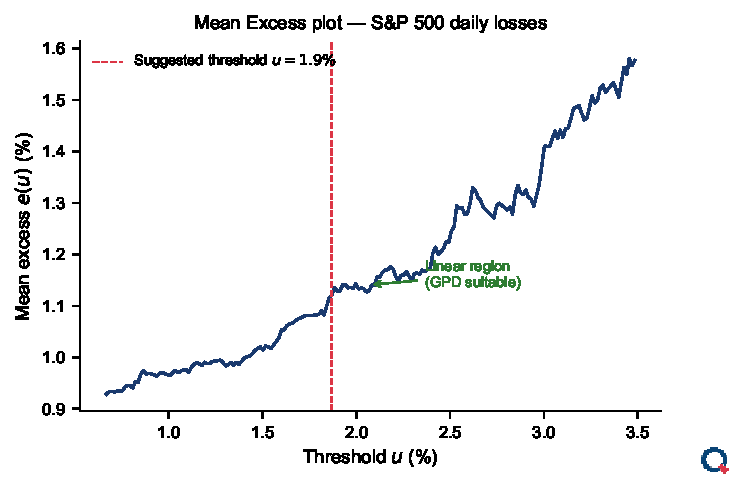
\includegraphics[width=\textwidth]{ch2_mean_excess_plot.pdf}
\end{center}
\end{column}
\begin{column}{0.52\textwidth}
\begin{block}{Funcția Mean Excess}
$$e(u) = \E[X - u \mid X > u] = \frac{\hat{\sigma} + \hat{\xi}u}{1 - \hat{\xi}}$$
\end{block}
\begin{itemize}\setlength{\itemsep}{0pt}
    \item Graficul $e(u)$ vs $u$: \textbf{linie dreaptă} dacă GPD este corectă
    \item Pantă pozitivă ($\hat{\xi} > 0$): cozi groase
    \item Pantă zero ($\hat{\xi} = 0$): cozi exponențiale
    \item \textbf{Prag optim:} zona unde graficul devine liniar
    \item Prag prea jos $\Rightarrow$ bias; prea sus $\Rightarrow$ varianță mare
\end{itemize}
\end{column}
\end{columns}
    \end{cminipage}
\end{frame}

\begin{frame}{Exercițiul 3: Estimatorul Hill}
    \begin{cminipage}{0.95\textwidth}
\begin{block}{Problemă}
\begin{itemize}\setlength{\itemsep}{0pt}
    \item Cele mai mari 6 pierderi zilnice (ordonate descrescător): $X_{(1)} = 8{,}2\%$, $X_{(2)} = 6{,}5\%$, $X_{(3)} = 5{,}1\%$, $X_{(4)} = 4{,}3\%$, $X_{(5)} = 3{,}8\%$, $X_{(6)} = 3{,}2\%$. Calculați $\hat{\alpha}_{\text{Hill}}$ pentru $k = 5$.
\end{itemize}
\end{block}

\begin{exampleblock}{Rezolvare}
\begin{itemize}\setlength{\itemsep}{0pt}
    \item $\hat{\xi}_{\text{Hill}} = \frac{1}{k}\sum_{i=1}^k \ln\frac{X_{(i)}}{X_{(k+1)}} = \frac{1}{5}\left[\ln\frac{8{,}2}{3{,}2} + \ln\frac{6{,}5}{3{,}2} + \ln\frac{5{,}1}{3{,}2} + \ln\frac{4{,}3}{3{,}2} + \ln\frac{3{,}8}{3{,}2}\right]$
    \item $= \frac{1}{5}[0{,}941 + 0{,}709 + 0{,}466 + 0{,}296 + 0{,}172] = \frac{2{,}584}{5} = 0{,}517$
    \item $\hat{\alpha}_{\text{Hill}} = 1/\hat{\xi}_{\text{Hill}} = 1/0{,}517 = \mathbf{1{,}93}$
    \item \textbf{Interpretare:} Indicele de coadă $\approx 2$ sugerează cozi foarte groase (varianță la limită). Consistent cu randamente financiare tipice ($\hat{\alpha} \in [2, 5]$).
\end{itemize}
\end{exampleblock}
    \end{cminipage}
\end{frame}

\begin{frame}{Graficul Hill --- Stabilitatea estimării}
    \begin{cminipage}{0.95\textwidth}
\quantlet{SFM\_ch2\_extreme\_value}{https://github.com/QuantLet/Stat_fin_markets/tree/master/Ch_02/SFM_ch2_extreme_value}

\begin{center}
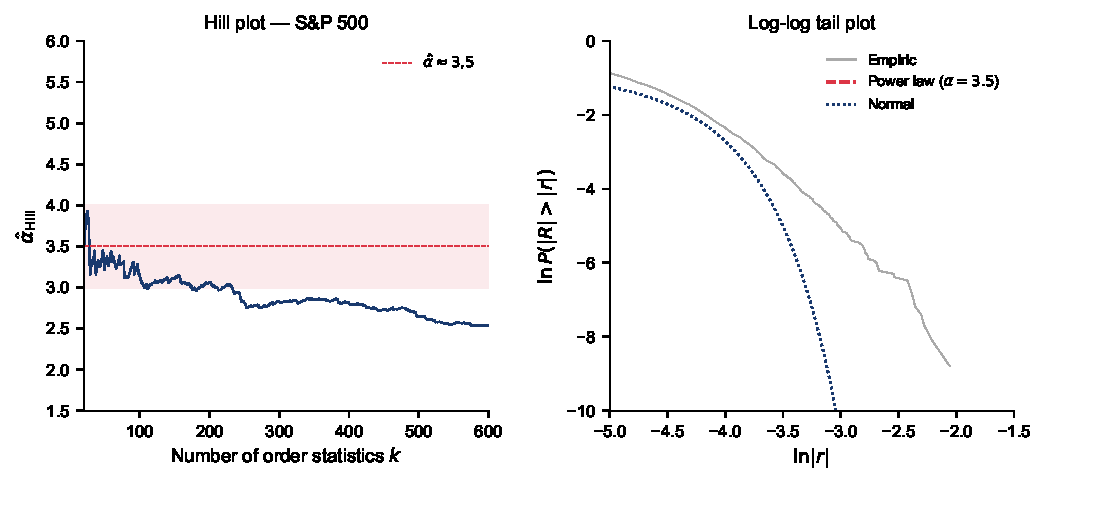
\includegraphics[width=0.7\textwidth]{ch2_hill_plot.pdf}
\end{center}

\vspace{-0.3cm}
\begin{itemize}\setlength{\itemsep}{0pt}
    \item $\hat{\alpha}_{\text{Hill}}^{(k)}$ vs.\ $k$: regiunea \textbf{stabilă} (platou) indică alegerea optimă a lui $k$
    \item $k$ mic: varianță mare (puține observații); $k$ mare: bias (include date non-extreme)
    \item \textbf{Regulă practică:} $k \in [50, 300]$ pentru $n \approx 2{.}500$ zile
\end{itemize}
    \end{cminipage}
\end{frame}

%=============================================================================
% PARTEA II: COMPARAREA DISTRIBUȚIILOR
%=============================================================================
\section{Partea II: Compararea distribuțiilor}

\begin{frame}{Exercițiul 4: AIC și BIC --- Selecția modelului}
    \begin{cminipage}{0.95\textwidth}
\begin{block}{Problemă}
\begin{itemize}\setlength{\itemsep}{0pt}
    \item Pe $n = 2{.}516$ randamente zilnice S\&P~500, MLE produce:
\end{itemize}
\renewcommand{\arraystretch}{1.1}
\begin{center}
\begin{tabular}{lccc}
\toprule
\textbf{Model} & \textbf{Parametri ($k$)} & $\boldsymbol{\ell}$ (log-lik) & \textbf{AIC} \\
\midrule
Normal & 2 & 7{,}890 & ? \\
Student-$t$ & 3 & 8{,}117 & ? \\
Skew-$t$ & 4 & 8{,}131 & ? \\
\bottomrule
\end{tabular}
\end{center}
\end{block}

\begin{exampleblock}{Rezolvare}
\small
\begin{itemize}\setlength{\itemsep}{0pt}
    \item Normal: $-15{,}776$; Student-$t$: $-16{,}228$; Skew-$t$: $\mathbf{-16{,}254}$ (cel mai bun)
    \item $\Delta\text{AIC}_{\text{Normal vs Skew-}t} = 478$ $\Rightarrow$ dovadă covârșitoare ($>10$ = puternic, $>100$ = indiscutabil)
\end{itemize}
\end{exampleblock}
    \end{cminipage}
\end{frame}

\begin{frame}{Comparație vizuală: Overlay și QQ-plot}
    \begin{cminipage}{0.95\textwidth}
\quantlet{SFM\_ch2\_dist\_comparison}{https://github.com/QuantLet/Stat_fin_markets/tree/master/Quantlets/SFM_ch2}

\begin{columns}[T]
\begin{column}{0.48\textwidth}
\begin{center}
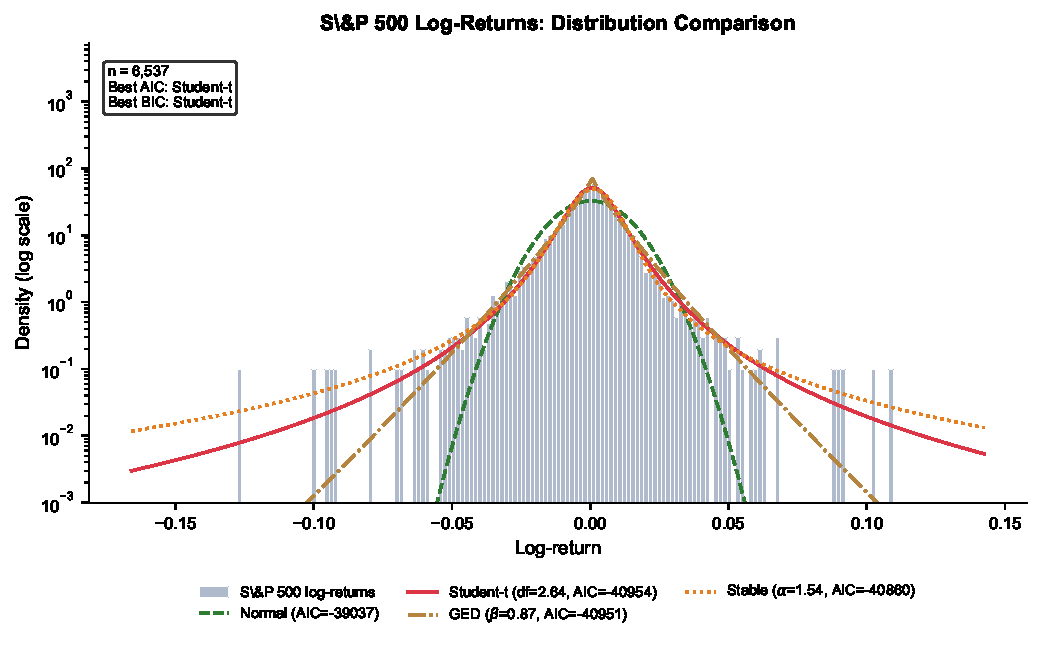
\includegraphics[height=0.45\textheight]{ch2_dist_comparison_overlay.pdf}\\
{\tiny Overlay: N vs $t$ vs Empiric}
\end{center}
\end{column}
\begin{column}{0.48\textwidth}
\begin{center}
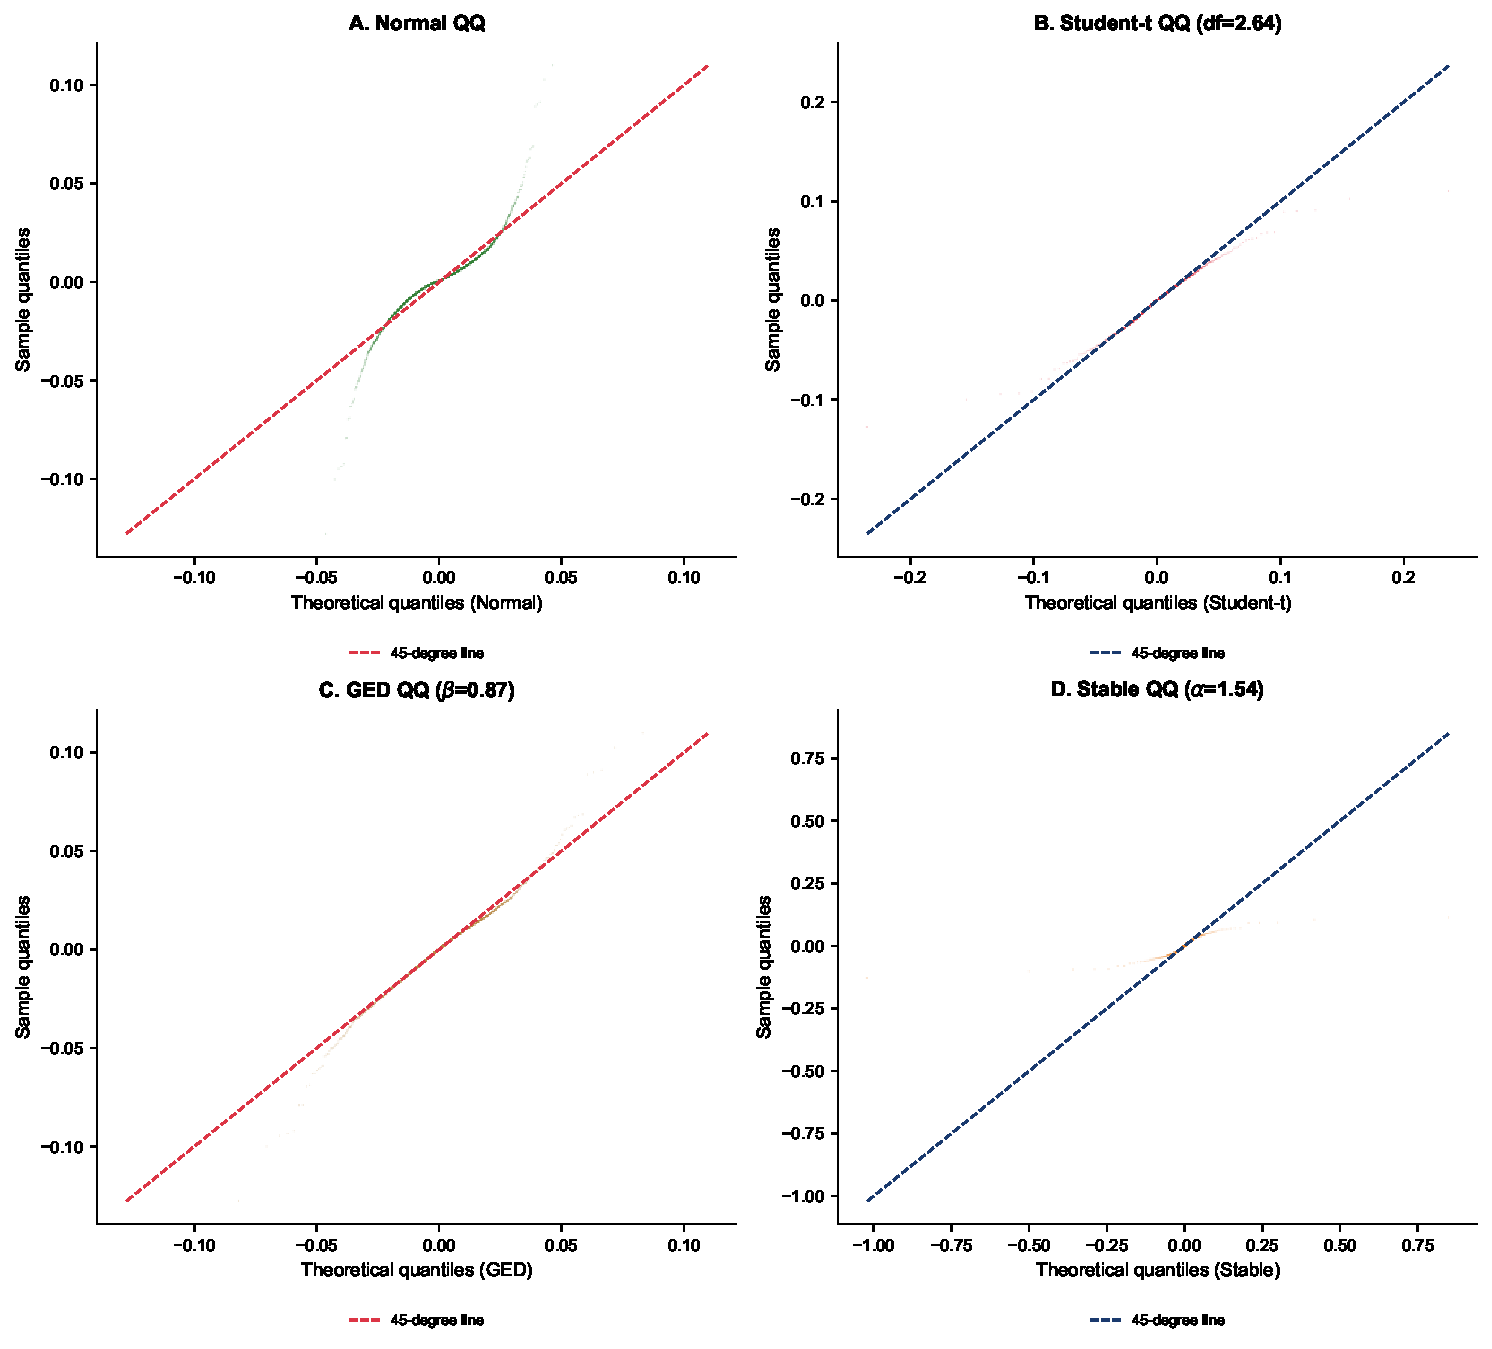
\includegraphics[height=0.45\textheight]{ch2_dist_comparison_qq.pdf}\\
{\tiny QQ-plot: devierea = inadecvare}
\end{center}
\end{column}
\end{columns}
\vspace{-0.1cm}
\footnotesize
\begin{itemize}\setlength{\itemsep}{0pt}
    \item Overlay: exces de kurtosis (vârf ascuțit + cozi groase)
    \item QQ-plot: curbură la capete $\Rightarrow$ cozi mai groase decât modelul
    \item \textbf{Diagnostic rapid:} QQ-plot este mai sensibil în cozi decât histograma
\end{itemize}
    \end{cminipage}
\end{frame}

\begin{frame}{Exercițiul 5: Backtesting VaR --- Testul Kupiec}
    \begin{cminipage}{0.95\textwidth}
\begin{block}{Problemă}
\begin{itemize}\setlength{\itemsep}{0pt}
    \item Un model VaR 1\% produce $v = 18$ depășiri pe $n = 1{,}000$ de zile. Testați validitatea modelului.
\end{itemize}
\end{block}

\begin{exampleblock}{Rezolvare}
\begin{itemize}\setlength{\itemsep}{0pt}
    \item Proporția observată: $\hat{p} = 18/1000 = 1{,}8\%$ vs așteptat $\alpha = 1\%$
    \item Testul Kupiec (Likelihood Ratio):
    $$LR = -2\ln\frac{\alpha^v(1-\alpha)^{n-v}}{\hat{p}^v(1-\hat{p})^{n-v}} = -2\ln\frac{0{,}01^{18} \cdot 0{,}99^{982}}{0{,}018^{18} \cdot 0{,}982^{982}}$$
    \item $LR = 7{,}35$; \quad $\chi^2_{1;\,0{,}05} = 3{,}84$
    \item $7{,}35 > 3{,}84$ $\Rightarrow$ \textbf{Respins}: modelul subestimează sistematic riscul de coadă
    \item \textbf{Concluzie:} 18 depășiri vs 10 așteptate --- modelul normal este inadecvat
\end{itemize}
\end{exampleblock}
    \end{cminipage}
\end{frame}

\begin{frame}{Backtesting vizual: VaR pe date reale}
    \begin{cminipage}{0.95\textwidth}
\quantlet{SFM\_ch2\_risk\_measures}{https://github.com/QuantLet/Stat_fin_markets/tree/master/Quantlets/SFM_ch2}

\begin{center}
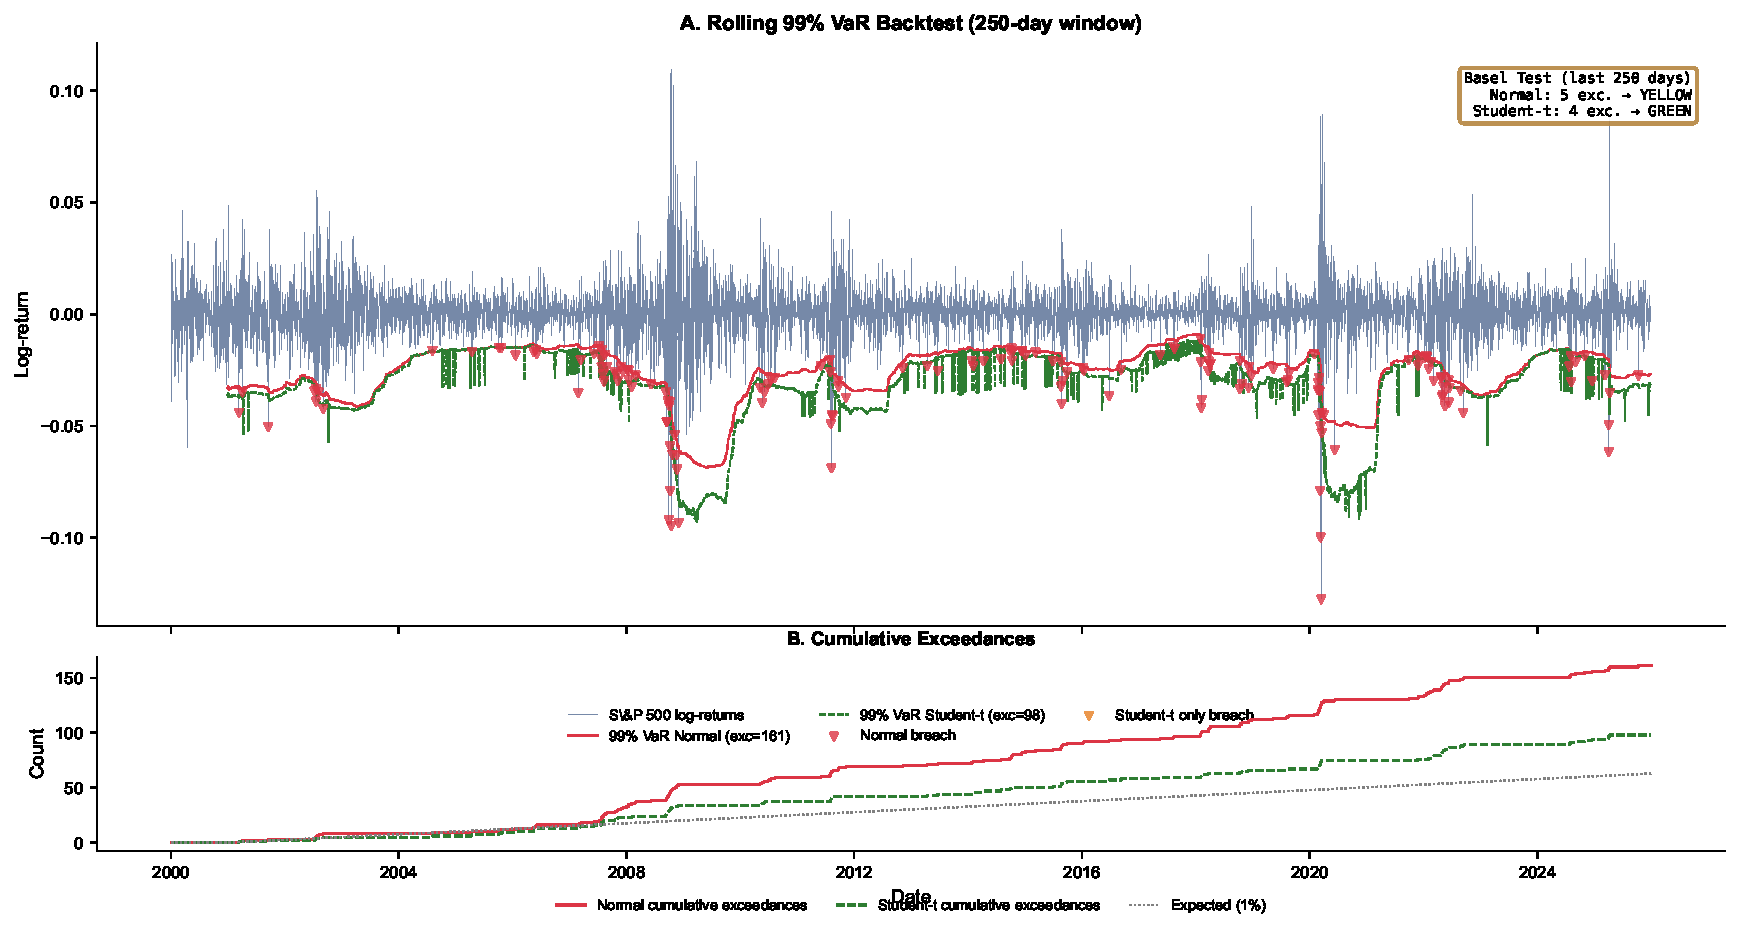
\includegraphics[width=0.65\textwidth]{ch2_var_backtest.pdf}
\end{center}
\vspace{-0.4cm}
\begin{itemize}\setlength{\itemsep}{0pt}
    \item Punctele \textcolor{Crimson}{roșii}: depășiri ale VaR (pierderi $>$ VaR estimat)
    \item Modelul normal (linia albastră) produce mai multe depășiri decât Student-$t$ sau EVT
    \item \textbf{Interpretare:} Un model bun produce $\sim\alpha\%$ depășiri, distribuite uniform
\end{itemize}
    \end{cminipage}
\end{frame}

%=============================================================================
% PARTEA III: COPULE
%=============================================================================
\section{Partea III: Copule}

\begin{frame}{Teorema lui Sklar --- Fundament}
    \begin{cminipage}{0.95\textwidth}
\begin{block}{Teoremă (Sklar, 1959)}
\begin{itemize}\setlength{\itemsep}{0pt}
    \item Orice distribuție multivariată $F(x_1, \ldots, x_d)$ cu marginale $F_1, \ldots, F_d$:
    $F(x_1, \ldots, x_d) = C(F_1(x_1), \ldots, F_d(x_d))$
    unde $C: [0,1]^d \to [0,1]$ este \textbf{copula}. Dacă marginalele sunt continue, $C$ este \textbf{unică}.
\end{itemize}
\end{block}
\vspace{0.1cm}
\begin{columns}[T]
\begin{column}{0.48\textwidth}
\begin{alertblock}{De ce copule?}
\begin{itemize}\setlength{\itemsep}{0pt}
    \item Separă structura marginală de structura de dependență
    \item Corelația Pearson $\rho$ captează doar dependența \textit{liniară}
    \item Copulele captează dependența \textit{de coadă} (crize!)
\end{itemize}
\end{alertblock}
\end{column}
\begin{column}{0.48\textwidth}
\begin{exampleblock}{Familii principale}
\begin{itemize}\setlength{\itemsep}{0pt}
    \item \textbf{Gaussiană:} $\lambda_U = \lambda_L = 0$ (fără dep.\ de coadă)
    \item \textbf{Student-$t$:} $\lambda_U = \lambda_L > 0$ (simetrică)
    \item \textbf{Clayton:} $\lambda_L > 0$, $\lambda_U = 0$ (coadă inferioară)
    \item \textbf{Gumbel:} $\lambda_U > 0$, $\lambda_L = 0$ (coadă superioară)
\end{itemize}
\end{exampleblock}
\end{column}
\end{columns}
    \end{cminipage}
\end{frame}

\begin{frame}{Exercițiul 6: Dependența de coadă --- Calcul}
    \begin{cminipage}{0.95\textwidth}
\begin{block}{Problemă}
\begin{itemize}\setlength{\itemsep}{0pt}
    \item Copula Student-$t$ bivariatăcu $\rho = 0{,}5$ și $\nu = 4$ grade de libertate. Calculați coeficientul de dependență de coadă $\lambda_U$.
\end{itemize}
\end{block}

\begin{exampleblock}{Rezolvare}
\begin{itemize}\setlength{\itemsep}{0pt}
    \item Formula: $\lambda_U = 2\,t_{\nu+1}\left(-\sqrt{\frac{(\nu+1)(1-\rho)}{1+\rho}}\right)$
    \item $\lambda_U = 2\,t_5\left(-\sqrt{\frac{5 \times 0{,}5}{1{,}5}}\right) = 2\,t_5\left(-\sqrt{1{,}667}\right) = 2\,t_5(-1{,}291)$
    \item $t_5(-1{,}291) \approx 0{,}127$ $\Rightarrow$ $\lambda_U = 2 \times 0{,}127 = \mathbf{0{,}254}$
    \item \textbf{Interpretare:} Dacă un activ suferă o pierdere extremă, probabilitatea ca celălalt activ să sufere simultan este $\sim$25\%. Sub copula Gaussiană, această probabilitate ar fi 0!
\end{itemize}
\end{exampleblock}
    \end{cminipage}
\end{frame}

\begin{frame}{Vizualizare: Copule pe date financiare}
    \begin{cminipage}{0.95\textwidth}
\quantlet{SFM\_ch2\_case\_study\_2c}{https://github.com/QuantLet/Stat_fin_markets/tree/master/Ch_02/SFM_ch2_case_study_2c}

\begin{center}
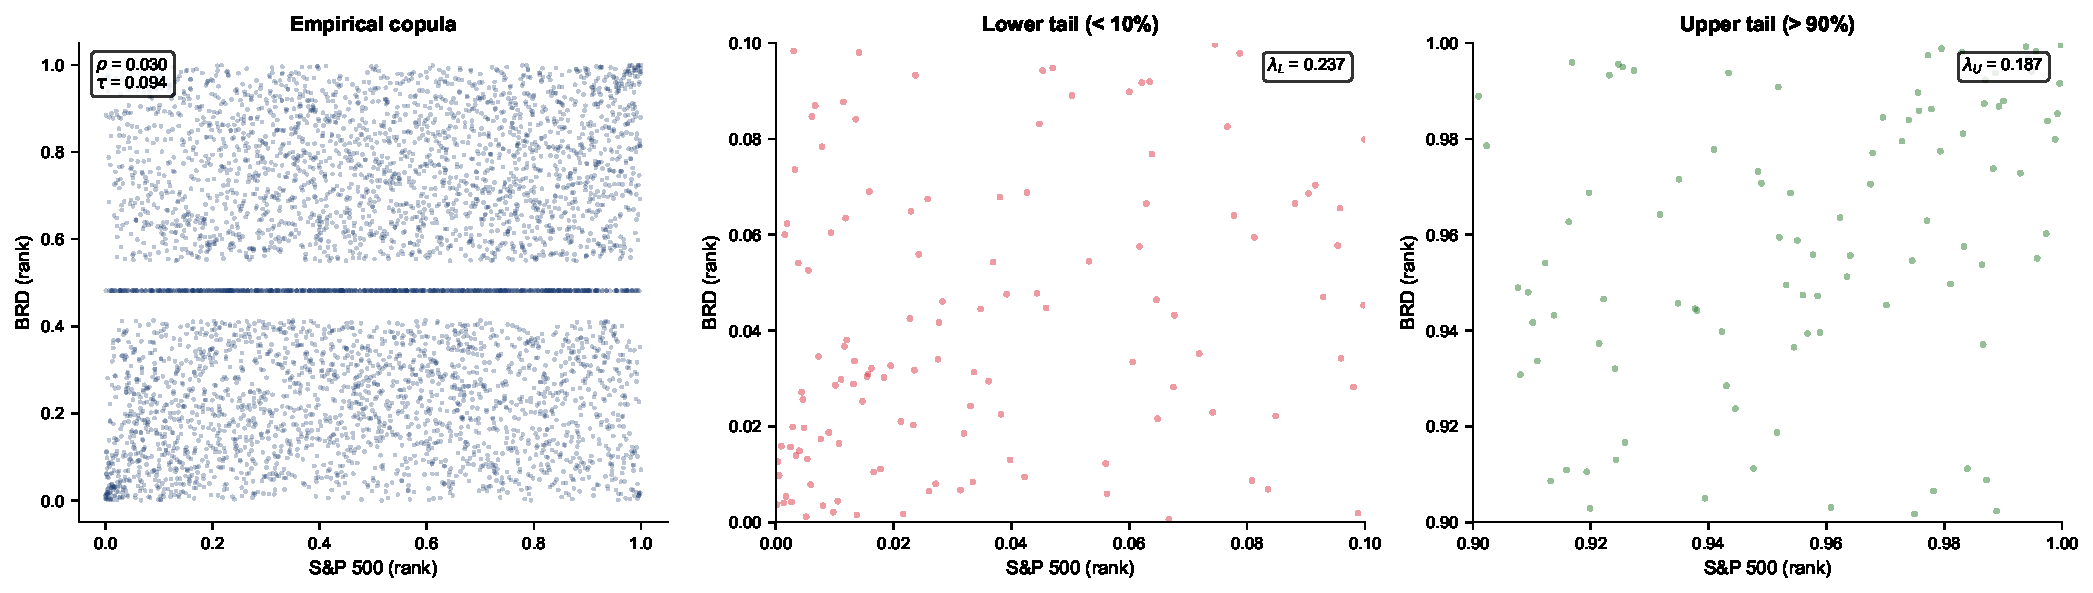
\includegraphics[width=0.65\textwidth]{ch2_cs2c_copula_scatter.pdf}
\end{center}
\vspace{-0.4cm}
\begin{itemize}\setlength{\itemsep}{0pt}
    \item Scatter-plot pe marginale uniforme ($U_1 = F_1(X_1)$, $U_2 = F_2(X_2)$)
    \item Concentrarea în colțurile $(0,0)$ și $(1,1)$: dependență de coadă
    \item Copula Gaussiană: concentrare centrală; Student-$t$: concentrare în colțuri
\end{itemize}
    \end{cminipage}
\end{frame}

\begin{frame}{Exercițiul 7: Alegerea copulei --- Tabel comparativ}
    \begin{cminipage}{0.95\textwidth}
\begin{block}{Problemă}
\begin{itemize}\setlength{\itemsep}{0pt}
    \item Date bivariate (S\&P~500, DAX). Ajustați 4 copule:
\end{itemize}
\renewcommand{\arraystretch}{1.1}
\begin{center}
\begin{tabular}{lcccc}
\toprule
\textbf{Copulă} & $\hat{\theta}$ & $\ell$ & \textbf{AIC} & $\hat{\lambda}_L$ \\
\midrule
Gaussiană & $\rho = 0{,}62$ & 312 & $-622$ & 0 \\
Student-$t$ & $\rho = 0{,}63$, $\nu = 6$ & 338 & $-672$ & 0{,}18 \\
Clayton & $\theta = 1{,}1$ & 305 & $-608$ & 0{,}22 \\
Gumbel & $\theta = 1{,}6$ & 295 & $-588$ & 0 \\
\bottomrule
\end{tabular}
\end{center}
\end{block}

\begin{exampleblock}{Rezolvare}
\small
\begin{itemize}\setlength{\itemsep}{0pt}
    \item \textbf{Cel mai bun AIC:} Student-$t$ ($-672$). $\Delta\text{AIC} = 50$ față de Gaussiană $\Rightarrow$ puternic
    \item Student-$t$: dep.\ de coadă simetrică ($\lambda_L = \lambda_U = 0{,}18$); Clayton: doar $\lambda_L$
    \item \textbf{Concluzie:} Copula Student-$t$ este preferabilă pentru portofolii diversificate
\end{itemize}
\end{exampleblock}
    \end{cminipage}
\end{frame}

%=============================================================================
% PARTEA IV: MANAGEMENTUL RISCULUI
%=============================================================================
\section{Partea IV: Managementul riscului}

\begin{frame}{Exercițiul 8: VaR și ES sub diferite distribuții}
    \begin{cminipage}{0.95\textwidth}
\begin{block}{Problemă}
\begin{itemize}\setlength{\itemsep}{0pt}
    \item Portofoliu de \$1M, $\mu = 0{,}03\%$/zi, $\sigma = 1{,}5\%$/zi. Calculați VaR și ES la 1\% sub: (a) distribuția normală; (b) Student-$t$ cu $\nu = 5$.
\end{itemize}
\end{block}

\begin{exampleblock}{Rezolvare}
\small
\renewcommand{\arraystretch}{1.1}
\begin{center}
\begin{tabular}{lcc}
\toprule
& \textbf{Normal} & \textbf{Student-$t$ ($\nu=5$)} \\
\midrule
VaR$_{1\%}$ & $3{,}52\%$ $\Rightarrow$ \textbf{\$35{,}190} & $3{,}93\%$ $\Rightarrow$ \textbf{\$39{,}330} \\
ES$_{1\%}$ & \$39{,}975 & \$52{,}100 \\
ES/VaR & 1{,}14 & 1{,}32 \\
\bottomrule
\end{tabular}
\end{center}
\begin{itemize}\setlength{\itemsep}{0pt}
    \item Student-$t$: factor $\sqrt{(\nu-2)/\nu} = 0{,}7746$ pe $\sigma$; cuantila $|t_{0{,}01;5}| = 3{,}365$ vs $z = 2{,}326$
    \item Cozile grele cresc ES relativ mai mult decât VaR
    \item \textbf{Basel III:} ES (nu VaR) este măsura oficială de risc de piață
\end{itemize}
\end{exampleblock}
    \end{cminipage}
\end{frame}

\begin{frame}{VaR: Subaditivitate și coerență}
    \begin{cminipage}{0.95\textwidth}
\quantlet{SFM\_ch2\_risk\_measures}{https://github.com/QuantLet/Stat_fin_markets/tree/master/Quantlets/SFM_ch2}

\begin{columns}[T]
\begin{column}{0.45\textwidth}
\begin{center}
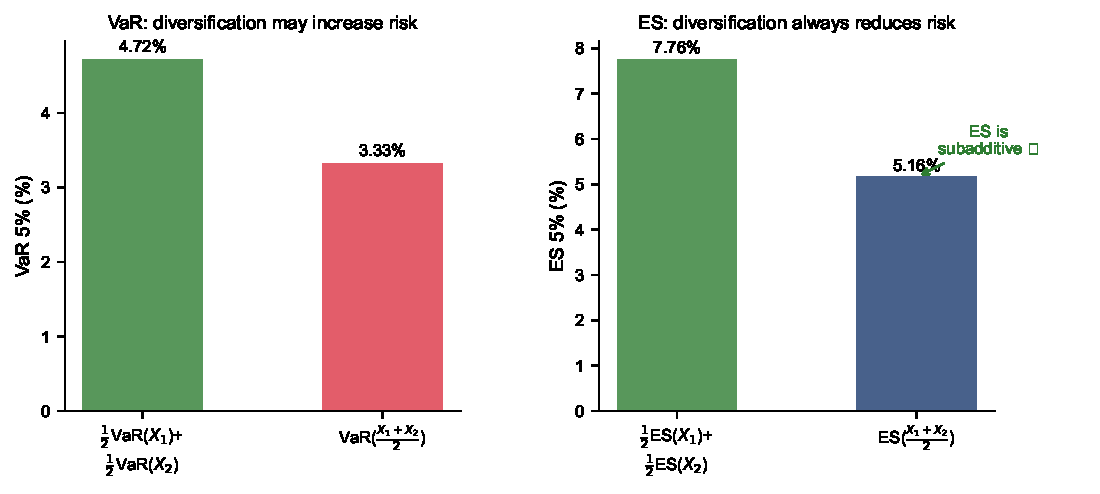
\includegraphics[width=0.95\textwidth]{ch2_var_subadditivity.pdf}
\end{center}
\end{column}
\begin{column}{0.52\textwidth}
\begin{alertblock}{VaR nu este subaditivă!}
\begin{itemize}\setlength{\itemsep}{0pt}
    \item Există cazuri unde:
    $$\text{VaR}(X+Y) > \text{VaR}(X) + \text{VaR}(Y)$$
    \item Diversificarea ``crește'' riscul?! $\Rightarrow$ Absurd
    \item VaR nu este măsură \textbf{coerentă} de risc
\end{itemize}
\end{alertblock}
\begin{exampleblock}{ES este subaditivă}
\begin{itemize}\setlength{\itemsep}{0pt}
    \item $\text{ES}(X+Y) \leq \text{ES}(X) + \text{ES}(Y)$
    \item ES satisface toate 4 axiomele Artzner (1999)
    \item De aceea Basel~III a trecut de la VaR la ES
\end{itemize}
\end{exampleblock}
\end{column}
\end{columns}
    \end{cminipage}
\end{frame}

\begin{frame}{Adevărat sau Fals? --- EVT, Copule și Risc}
\begin{cminipage}{0.95\textwidth}
    \small
    \begin{enumerate}\setlength{\itemsep}{-1pt}
        \item $\hat{\xi} > 0$ în GEV indică cozi groase de tip Fréchet.
        \item Metoda POT necesită împărțirea datelor în blocuri.
        \item Copula Gaussiană captează dependența de coadă.
        \item ES este întotdeauna $\geq$ VaR la același nivel de încredere.
        \item BIC penalizează mai puternic decât AIC pentru $n > 8$.
        \item Estimatorul Hill funcționează doar pentru cozi de tip lege putere.
        \item Testul Kupiec evaluează dacă numărul de depășiri VaR este consistent cu $\alpha$.
    \end{enumerate}
    \vspace{0.1cm}
    \begin{exampleblock}{Răspunsuri}
    \scriptsize
    \begin{enumerate}\setlength{\itemsep}{0pt}
        \item \correct\ \textbf{A}: Fréchet = lege putere; Gumbel ($\xi=0$); Weibull ($\xi<0$)
        \item \incorrect\ \textbf{F}: POT = depășiri peste prag, nu blocuri. Block Maxima = blocuri
        \item \incorrect\ \textbf{F}: Gaussiana: $\lambda_U = \lambda_L = 0$. Trebuie Student-$t$ sau Arhimediană
        \item \correct\ \textbf{A}: ES $=$ media pierderilor $\mid$ pierdere $>$ VaR $\Rightarrow$ ES $\geq$ VaR
        \item \correct\ \textbf{A}: BIC: $k\ln n$; AIC: $2k$. $\ln n > 2$ pentru $n > 8$
        \item \correct\ \textbf{A}: Hill presupune $P(X > x) \sim Cx^{-\alpha}$
        \item \correct\ \textbf{A}: Kupiec: $H_0: p = \alpha$ cu LR $\sim \chi^2(1)$
    \end{enumerate}
    \end{exampleblock}
\end{cminipage}
\end{frame}

%=============================================================================
% PARTEA V: PYTHON
%=============================================================================
\section{Partea V: Python}

\begin{frame}[fragile]{Lab 1: EVT și backtesting VaR}
    \begin{cminipage}{0.95\textwidth}
\quantlet{SFM\_ch2\_extreme\_value}{https://github.com/QuantLet/Stat_fin_markets/tree/master/Ch_02/SFM_ch2_extreme_value}

\begin{block}{Exercițiu Python (30 min)}
\small
Deschideți \texttt{SFM\_ch2\_extreme\_value.ipynb}:
\begin{enumerate}\setlength{\itemsep}{0pt}
    \item Descărcați randamente S\&P~500 (2015--2025); grafic Mean Excess $\Rightarrow$ alegeți $u$
    \item Ajustați GPD pe excese $\Rightarrow$ $(\hat{\xi}, \hat{\sigma})$; calculați VaR/ES la 1\%
    \item Comparați cu VaR/ES sub normală și Student-$t$
    \item Backtest VaR cu fereastră mobilă 250 zile; testul Kupiec
\end{enumerate}
\end{block}

\begin{lstlisting}
from scipy.stats import genpareto
# Fit GPD on exceedances
excess = losses[losses > u] - u
xi, loc, sigma = genpareto.fit(excess, floc=0)
print(f"xi = {xi:.3f}, sigma = {sigma:.4f}")
# VaR POT
VaR = u + (sigma/xi) * ((n*alpha/Nu)**(-xi) - 1)
\end{lstlisting}
    \end{cminipage}
\end{frame}

\begin{frame}[fragile]{Lab 2: Copule în Python}
    \begin{cminipage}{0.95\textwidth}
\begin{exampleblock}{Exercițiu Python (20 min)}
\small
Analizați dependența S\&P~500 -- DAX:
\begin{enumerate}\setlength{\itemsep}{0pt}
    \item Randamente zilnice $\Rightarrow$ marginale uniforme (PIT)
    \item Ajustați copule: Gaussiană, Student-$t$, Clayton, Gumbel
    \item Comparați AIC; estimați $\lambda_L$, $\lambda_U$; scatter-plot $[0,1]^2$
\end{enumerate}
\end{exampleblock}

\begin{lstlisting}
from copulas.bivariate import Clayton, Gumbel
from scipy.stats import kendalltau
# Kendall's tau -> theta
tau, _ = kendalltau(u1, u2)
# Clayton: theta = 2*tau/(1-tau)
theta_c = 2 * tau / (1 - tau)
lambda_L = 2**(-1/theta_c)  # lower tail dependence
print(f"Clayton: theta={theta_c:.2f}, lambda_L={lambda_L:.3f}")
\end{lstlisting}
    \end{cminipage}
\end{frame}

\begin{frame}[fragile]{Lab 3: GARCH cu inovații non-Gaussiene}
    \begin{cminipage}{0.95\textwidth}
\quantlet{SFM\_ch2\_modern\_extensions}{https://github.com/QuantLet/Stat_fin_markets/tree/master/Ch_02/SFM_ch2_modern_extensions}

\begin{block}{Exercițiu Python (15 min)}
Comparați GARCH(1,1) cu diferite inovații:
\begin{enumerate}\setlength{\itemsep}{2pt}
    \item Ajustați GARCH(1,1) cu inovații normale și Student-$t$
    \item Comparați AIC/BIC
    \item Extrageți reziduurile standardizate: sunt i.i.d.?
    \item Calculați VaR 1\% \textbf{condiționat} pe volatilitatea curentă
\end{enumerate}
\end{block}

\begin{lstlisting}
from arch import arch_model
# GARCH(1,1) with Student-t innovations
model = arch_model(returns, vol='Garch', p=1, q=1, dist='t')
res = model.fit(disp='off')
# Conditional VaR
cond_vol = res.conditional_volatility
VaR_t = res.params['mu'] + cond_vol * t.ppf(0.01, res.params['nu'])
\end{lstlisting}
    \end{cminipage}
\end{frame}

%=============================================================================
% DISCUȚII ȘI AI
%=============================================================================
\section{Discuții și AI}

\begin{frame}{Scenarii practice: Ce model alegeți?}
    \begin{cminipage}{0.95\textwidth}
\begin{block}{Scenariul 1: Fond de investiții --- raportare zilnică}
\begin{itemize}\setlength{\itemsep}{0pt}
    \item Portofoliu diversificat (acțiuni, obligațiuni, FX). Trebuie VaR zilnic la 1\%.
    \item \textbf{Recomandare:} GARCH(1,1) cu inovații Student-$t$ --- captează clusterizarea volatilității și cozile groase
\end{itemize}
\end{block}

\begin{exampleblock}{Scenariul 2: Bancă --- cerințe de capital Basel~III}
\begin{itemize}\setlength{\itemsep}{0pt}
    \item Regulatorul cere ES la 2{,}5\% pe orizont de 10 zile.
    \item \textbf{Recomandare:} EVT (POT) pe reziduurile GARCH --- cel mai robust pentru cozi extreme
\end{itemize}
\end{exampleblock}

\begin{alertblock}{Scenariul 3: Asigurări --- modelarea pierderilor catastrofale}
\begin{itemize}\setlength{\itemsep}{0pt}
    \item Pierderi rare dar extreme (cutremure, inundații). Dependență spațială.
    \item \textbf{Recomandare:} EVT + copule Clayton/Gumbel pentru dependența de coadă
\end{itemize}
\end{alertblock}
    \end{cminipage}
\end{frame}

\begin{frame}{Exercițiu AI: Verificați codul generat}
    \begin{cminipage}{0.95\textwidth}
\begin{alertblock}{Prompt pentru AI}
\small
``Scrie cod Python care ajustează GPD pe excesele peste pragul $u=2{,}5\%$ din randamentele S\&P~500 și calculează VaR la 1\%.''
\end{alertblock}

\vspace{0.2cm}
\begin{block}{Ce trebuie verificat:}
\begin{enumerate}\setlength{\itemsep}{2pt}
    \item \textbf{Semnul randamentelor:} AI-ul a folosit pierderi ($-r_t$) sau randamente ($r_t$)?
    \item \textbf{Parametrul \texttt{floc=0}:} GPD trebuie ajustat cu locație fixă la 0 (excesele sunt deja centrate)
    \item \textbf{Formula VaR POT:} verificați dacă folosește $n/N_u$ corect, nu $N_u/n$
    \item \textbf{Pragul $u$:} este selectat prin Mean Excess plot sau arbitrar?
    \item \textbf{Interpretare:} VaR-ul returnat este zilnic sau anual? Procent sau valoare absolută?
\end{enumerate}
\end{block}

\begin{itemize}\setlength{\itemsep}{0pt}
    \item \textbf{Regulă:} Codul AI poate fi un punct de \textit{plecare}, nu un produs finit. Verificați \textbf{întotdeauna} convențiile de semn și formulele!
\end{itemize}
    \end{cminipage}
\end{frame}

%=============================================================================
% TEST RAPID
%=============================================================================
\section{Test rapid}

\begin{frame}{Test 1: GPD și POT}
\begin{cminipage}{0.95\textwidth}
    \begin{alertblock}{Întrebare}
        \begin{itemize}\setlength{\itemsep}{0pt}
            \item În metoda POT, ce distribuție se ajustează pe excesele peste prag?
        \end{itemize}
    \end{alertblock}

    \vspace{0.3cm}

    \begin{block}{Variante de răspuns}
        \textcolor{MainBlue}{\textbf{(A)}} Distribuția normală\\[3pt]
        \textcolor{MainBlue}{\textbf{(B)}} Distribuția Pareto generalizată (GPD)\\[3pt]
        \textcolor{MainBlue}{\textbf{(C)}} Distribuția exponențială\\[3pt]
        \textcolor{MainBlue}{\textbf{(D)}} Distribuția GEV
    \end{block}
\end{cminipage}
\end{frame}

\begin{frame}{Test 1: Răspuns}
\begin{cminipage}{0.95\textwidth}
    \begin{exampleblock}{Răspuns: B}
        Teorema Pickands--Balkema--de Haan: excesele peste un prag $u$ suficient de mare converg la GPD.
    \end{exampleblock}

    \vspace{0.2cm}

    \begin{itemize}\setlength{\itemsep}{0pt}
        \item \textbf{A} --- Normala nu modelează cozi extreme \incorrect
        \item \textbf{C} --- Exponențiala este GPD cu $\xi = 0$ (caz particular, prea restrictiv) \incorrect
        \item \textbf{D} --- GEV este pentru Block Maxima, nu POT \incorrect
    \end{itemize}
\end{cminipage}
\end{frame}

\begin{frame}{Test 2: Estimatorul Hill}
\begin{cminipage}{0.95\textwidth}
    \begin{alertblock}{Întrebare}
        \begin{itemize}\setlength{\itemsep}{0pt}
            \item Ce presupunere fundamentală face estimatorul Hill despre coada distribuției?
        \end{itemize}
    \end{alertblock}

    \vspace{0.3cm}

    \begin{block}{Variante de răspuns}
        \textcolor{MainBlue}{\textbf{(A)}} Coada scade exponențial\\[3pt]
        \textcolor{MainBlue}{\textbf{(B)}} Coada urmează o lege putere: $P(X > x) \sim Cx^{-\alpha}$\\[3pt]
        \textcolor{MainBlue}{\textbf{(C)}} Distribuția este simetrică\\[3pt]
        \textcolor{MainBlue}{\textbf{(D)}} Distribuția are varianță finită
    \end{block}
\end{cminipage}
\end{frame}

\begin{frame}{Test 2: Răspuns}
\begin{cminipage}{0.95\textwidth}
    \begin{exampleblock}{Răspuns: B}
        Hill este un estimator \textbf{semi-parametric} care presupune variație regulată (lege putere) în coada dreaptă.
    \end{exampleblock}

    \vspace{0.2cm}

    \begin{itemize}\setlength{\itemsep}{0pt}
        \item \textbf{A} --- Cozi exponențiale: Hill nu este aplicabil (dă $\hat{\alpha} \to \infty$) \incorrect
        \item \textbf{C} --- Nu necesită simetrie, funcționează pe o singură coadă \incorrect
        \item \textbf{D} --- Funcționează chiar și cu varianță infinită ($\alpha < 2$) \incorrect
    \end{itemize}
\end{cminipage}
\end{frame}

\begin{frame}{Test 3: Copula și dependența de coadă}
\begin{cminipage}{0.95\textwidth}
    \begin{alertblock}{Întrebare}
        \begin{itemize}\setlength{\itemsep}{0pt}
            \item Care copulă are dependență de coadă \textbf{simetrică} ($\lambda_L = \lambda_U > 0$)?
        \end{itemize}
    \end{alertblock}

    \vspace{0.3cm}

    \begin{block}{Variante de răspuns}
        \textcolor{MainBlue}{\textbf{(A)}} Gaussiană\\[3pt]
        \textcolor{MainBlue}{\textbf{(B)}} Clayton\\[3pt]
        \textcolor{MainBlue}{\textbf{(C)}} Student-$t$\\[3pt]
        \textcolor{MainBlue}{\textbf{(D)}} Gumbel
    \end{block}
\end{cminipage}
\end{frame}

\begin{frame}{Test 3: Răspuns}
\begin{cminipage}{0.95\textwidth}
    \begin{exampleblock}{Răspuns: C}
        Copula Student-$t$ are $\lambda_L = \lambda_U > 0$. Dependența de coadă crește cu scăderea lui $\nu$.
    \end{exampleblock}

    \vspace{0.2cm}

    \begin{itemize}\setlength{\itemsep}{0pt}
        \item \textbf{A} --- Gaussiana: $\lambda_L = \lambda_U = 0$ (nicio dependență de coadă) \incorrect
        \item \textbf{B} --- Clayton: doar $\lambda_L > 0$ (asimetrică, coada inferioară) \incorrect
        \item \textbf{D} --- Gumbel: doar $\lambda_U > 0$ (asimetrică, coada superioară) \incorrect
    \end{itemize}
\end{cminipage}
\end{frame}

\begin{frame}{Test 4: VaR vs ES}
\begin{cminipage}{0.95\textwidth}
    \begin{alertblock}{Întrebare}
        \begin{itemize}\setlength{\itemsep}{0pt}
            \item De ce Basel~III a înlocuit VaR cu ES ca măsură principală de risc de piață?
        \end{itemize}
    \end{alertblock}

    \vspace{0.3cm}

    \begin{block}{Variante de răspuns}
        \textcolor{MainBlue}{\textbf{(A)}} ES este mai ușor de calculat\\[3pt]
        \textcolor{MainBlue}{\textbf{(B)}} ES este subaditivă (coerentă) și captează gravitatea cozii\\[3pt]
        \textcolor{MainBlue}{\textbf{(C)}} VaR subestimează întotdeauna riscul\\[3pt]
        \textcolor{MainBlue}{\textbf{(D)}} ES este mai stabilă la alegerea nivelului de încredere
    \end{block}
\end{cminipage}
\end{frame}

\begin{frame}{Test 4: Răspuns}
\begin{cminipage}{0.95\textwidth}
    \begin{exampleblock}{Răspuns: B}
        ES satisface subaditivitatea: diversificarea reduce riscul. VaR poate penaliza diversificarea.
    \end{exampleblock}

    \vspace{0.2cm}

    \begin{itemize}\setlength{\itemsep}{0pt}
        \item \textbf{A} --- ES este de fapt \textit{mai greu} de calculat (necesită integrale) \incorrect
        \item \textbf{C} --- VaR nu subestimează \textit{întotdeauna}; problema este non-coerența \incorrect
        \item \textbf{D} --- Stabilitatea nu este motivul principal al schimbării regulamentare \incorrect
    \end{itemize}
\end{cminipage}
\end{frame}

\begin{frame}{Test 5: Testul Kupiec}
\begin{cminipage}{0.95\textwidth}
    \begin{alertblock}{Întrebare}
        \begin{itemize}\setlength{\itemsep}{0pt}
            \item Un model VaR 1\% produce 35 depășiri pe 2{,}000 de zile. Așteptarea: 20. Ce concluzie trageți?
        \end{itemize}
    \end{alertblock}

    \vspace{0.3cm}

    \begin{block}{Variante de răspuns}
        \textcolor{MainBlue}{\textbf{(A)}} Modelul este acceptabil (35 $\approx$ 20)\\[3pt]
        \textcolor{MainBlue}{\textbf{(B)}} Modelul subestimează riscul semnificativ\\[3pt]
        \textcolor{MainBlue}{\textbf{(C)}} Modelul supraestimează riscul\\[3pt]
        \textcolor{MainBlue}{\textbf{(D)}} Nu putem concluziona fără BIC
    \end{block}
\end{cminipage}
\end{frame}

\begin{frame}{Test 5: Răspuns}
\begin{cminipage}{0.95\textwidth}
    \begin{exampleblock}{Răspuns: B}
        $\hat{p} = 35/2000 = 1{,}75\%$ vs $\alpha = 1\%$. Modelul produce $1{,}75\times$ mai multe depășiri.
    \end{exampleblock}

    \vspace{0.2cm}

    \begin{itemize}\setlength{\itemsep}{0pt}
        \item Kupiec: $LR = -2\ln\frac{0{,}01^{35} \cdot 0{,}99^{1965}}{0{,}0175^{35} \cdot 0{,}9825^{1965}} = 9{,}12 > 3{,}84$
        \item $\Rightarrow$ \textbf{Respins} la 5\%: modelul subestimează sistematic riscul
        \item \textbf{A} --- 35 vs 20 nu este ``aproape'' \incorrect
        \item \textbf{C} --- Mai multe depășiri = model prea optimist, nu prea conservator \incorrect
        \item \textbf{D} --- BIC este pentru selecția modelului, nu backtesting \incorrect
    \end{itemize}
\end{cminipage}
\end{frame}

\begin{frame}{Test 6: AIC vs BIC}
\begin{cminipage}{0.95\textwidth}
    \begin{alertblock}{Întrebare}
        \begin{itemize}\setlength{\itemsep}{0pt}
            \item Modelul A: AIC $= 5{,}200$. Modelul B: AIC $= 5{,}180$. Care este mai bun și cât de puternică este dovada?
        \end{itemize}
    \end{alertblock}

    \vspace{0.3cm}

    \begin{block}{Variante de răspuns}
        \textcolor{MainBlue}{\textbf{(A)}} A este mai bun (AIC mai mare)\\[3pt]
        \textcolor{MainBlue}{\textbf{(B)}} B este mai bun, dovadă puternică ($\Delta > 10$)\\[3pt]
        \textcolor{MainBlue}{\textbf{(C)}} B este mai bun, dar diferența nu este semnificativă\\[3pt]
        \textcolor{MainBlue}{\textbf{(D)}} Nu putem compara modele diferite cu AIC
    \end{block}
\end{cminipage}
\end{frame}

\begin{frame}{Test 6: Răspuns}
\begin{cminipage}{0.95\textwidth}
    \begin{exampleblock}{Răspuns: B}
        $\Delta\text{AIC} = 5{,}200 - 5{,}180 = 20 > 10$ $\Rightarrow$ dovadă puternică pentru modelul B.
    \end{exampleblock}

    \vspace{0.2cm}

    \begin{itemize}\setlength{\itemsep}{0pt}
        \item Scala Burnham--Anderson: $\Delta < 2$ slab; $4$--$7$ moderat; $> 10$ puternic
        \item \textbf{A} --- Confundă direcția: AIC \textit{mai mic} = mai bun \incorrect
        \item \textbf{C} --- $\Delta = 20$ este deasupra pragului de semnificație \incorrect
        \item \textbf{D} --- AIC poate compara orice modele pe aceleași date \incorrect
    \end{itemize}
\end{cminipage}
\end{frame}

\begin{frame}{Test 7: Mean Excess plot}
\begin{cminipage}{0.95\textwidth}
    \begin{alertblock}{Întrebare}
        \begin{itemize}\setlength{\itemsep}{0pt}
            \item Graficul Mean Excess $e(u)$ vs $u$ are pantă pozitivă. Ce implică aceasta?
        \end{itemize}
    \end{alertblock}

    \vspace{0.3cm}

    \begin{block}{Variante de răspuns}
        \textcolor{MainBlue}{\textbf{(A)}} Distribuția are cozi exponențiale\\[3pt]
        \textcolor{MainBlue}{\textbf{(B)}} Distribuția are cozi groase ($\xi > 0$)\\[3pt]
        \textcolor{MainBlue}{\textbf{(C)}} Distribuția este simetrică\\[3pt]
        \textcolor{MainBlue}{\textbf{(D)}} Pragul ales este prea mare
    \end{block}
\end{cminipage}
\end{frame}

\begin{frame}{Test 7: Răspuns}
\begin{cminipage}{0.95\textwidth}
    \begin{exampleblock}{Răspuns: B}
        $e(u) = (\hat{\sigma} + \hat{\xi}u)/(1 - \hat{\xi})$. Pantă pozitivă $\Leftrightarrow$ $\hat{\xi} > 0$ $\Leftrightarrow$ cozi groase (Fréchet).
    \end{exampleblock}

    \vspace{0.2cm}

    \begin{itemize}\setlength{\itemsep}{0pt}
        \item \textbf{A} --- Cozi exponențiale: $e(u) = \text{const}$ (pantă zero, $\xi = 0$) \incorrect
        \item \textbf{C} --- Mean Excess nu informează despre simetrie \incorrect
        \item \textbf{D} --- Pragul nu afectează \textit{panta}, doar volatilitatea estimării \incorrect
    \end{itemize}
\end{cminipage}
\end{frame}

\begin{frame}{Test 8: Teorema lui Sklar}
\begin{cminipage}{0.95\textwidth}
    \begin{alertblock}{Întrebare}
        \begin{itemize}\setlength{\itemsep}{0pt}
            \item Ce garantează Teorema lui Sklar despre unicitatea copulei?
        \end{itemize}
    \end{alertblock}

    \vspace{0.3cm}

    \begin{block}{Variante de răspuns}
        \textcolor{MainBlue}{\textbf{(A)}} Copula este unică pentru orice distribuție multivariată\\[3pt]
        \textcolor{MainBlue}{\textbf{(B)}} Copula este unică dacă marginalele sunt continue\\[3pt]
        \textcolor{MainBlue}{\textbf{(C)}} Copula este unică doar pentru distribuții eliptice\\[3pt]
        \textcolor{MainBlue}{\textbf{(D)}} Copula nu este niciodată unică
    \end{block}
\end{cminipage}
\end{frame}

\begin{frame}{Test 8: Răspuns}
\begin{cminipage}{0.95\textwidth}
    \begin{exampleblock}{Răspuns: B}
        Sklar (1959): dacă $F_1, \ldots, F_d$ sunt continue, copula $C$ este \textbf{unică}. Pentru marginale discrete, copula nu este neapărat unică.
    \end{exampleblock}

    \vspace{0.2cm}

    \begin{itemize}\setlength{\itemsep}{0pt}
        \item \textbf{A} --- Nu ``orice'': necesită continuitate \incorrect
        \item \textbf{C} --- Nu doar eliptice: funcționează pentru orice marginale continue \incorrect
        \item \textbf{D} --- Este unică sub continuitate \incorrect
    \end{itemize}
\end{cminipage}
\end{frame}

%=============================================================================
% REZUMAT
%=============================================================================
\section{Rezumat}

\begin{frame}{Checklist: Ce trebuie să știți}
    \begin{cminipage}{0.95\textwidth}
\begin{columns}[T]
\begin{column}{0.48\textwidth}
\begin{block}{EVT}
\begin{itemize}\setlength{\itemsep}{0pt}
    \item[$\square$] GEV: Fréchet ($\xi > 0$), Gumbel ($\xi = 0$), Weibull ($\xi < 0$)
    \item[$\square$] GPD: ajustare pe excese peste prag $u$
    \item[$\square$] Formulele VaR POT și ES POT
    \item[$\square$] Mean Excess plot: alegerea pragului
    \item[$\square$] Hill: indicele de coadă, graficul Hill
\end{itemize}
\end{block}
\begin{block}{Copule}
\begin{itemize}\setlength{\itemsep}{0pt}
    \item[$\square$] Teorema lui Sklar
    \item[$\square$] Gaussiană vs Student-$t$: $\lambda_U$
    \item[$\square$] Clayton ($\lambda_L$) vs Gumbel ($\lambda_U$)
    \item[$\square$] AIC pentru selecția copulei
\end{itemize}
\end{block}
\end{column}
\begin{column}{0.48\textwidth}
\begin{block}{Selecția modelului}
\begin{itemize}\setlength{\itemsep}{0pt}
    \item[$\square$] AIC: $-2\ell + 2k$
    \item[$\square$] BIC: $-2\ell + k\ln n$
    \item[$\square$] QQ-plot: interpretare
    \item[$\square$] Scala $\Delta$AIC: 2/4--7/10+
\end{itemize}
\end{block}
\begin{block}{Managementul riscului}
\begin{itemize}\setlength{\itemsep}{0pt}
    \item[$\square$] VaR: definiție, calcul
    \item[$\square$] ES: subaditivitate, coerență
    \item[$\square$] Kupiec: LR, $\chi^2(1)$
    \item[$\square$] Basel III: ES $>$ VaR
    \item[$\square$] GARCH + inovații non-Gaussiene
\end{itemize}
\end{block}
\end{column}
\end{columns}
    \end{cminipage}
\end{frame}

\begin{frame}{Tema pentru acasă}
    \begin{cminipage}{0.95\textwidth}
\begin{alertblock}{Exercițiu individual (deadline: următorul seminar)}
\begin{enumerate}\setlength{\itemsep}{3pt}
    \item Alegeți un activ financiar (acțiune, criptomonedă, FX) cu minim 5 ani de date zilnice
    \item Aplicați metoda POT: grafic Mean Excess $\Rightarrow$ alegeți $u$ $\Rightarrow$ ajustați GPD
    \item Calculați VaR 1\% și ES 1\% sub 3 modele: Normal, Student-$t$, EVT
    \item Efectuați backtesting VaR pe ultimii 2 ani (fereastră mobilă 250 zile)
    \item Raportați: tabel comparativ, graficul Hill, Mean Excess, testul Kupiec
    \item \textbf{Bonus:} ajustați o copulă Student-$t$ pe perechea activ ales + S\&P~500
\end{enumerate}
\end{alertblock}

\begin{exampleblock}{Resurse}
\begin{itemize}\setlength{\itemsep}{0pt}
    \item Quantlet: \url{https://github.com/QuantLet/Stat_fin_markets/tree/master/Ch_02}
    \item Curs: \url{https://danpele.github.io/SFM/}
\end{itemize}
\end{exampleblock}
    \end{cminipage}
\end{frame}

%=============================================================================
% BIBLIOGRAFIE
%=============================================================================
\section{Bibliografie}

\begin{frame}{Bibliografie}
    \begin{cminipage}{0.95\textwidth}
    \begin{block}{Referințe principale}
        {\small
        \begin{itemize}\setlength{\itemsep}{0pt}
            \item Embrechts, P., Kl\"{u}ppelberg, C., Mikosch, T. (1997). \textit{Modelling Extremal Events for Insurance and Finance}, Springer.
            \item McNeil, A.J., Frey, R., Embrechts, P. (2015). \textit{Quantitative Risk Management}, 2nd ed., Princeton.
            \item Nelsen, R.B. (2006). \textit{An Introduction to Copulas}, 2nd ed., Springer.
            \item de Haan, L., Ferreira, A. (2006). \textit{Extreme Value Theory: An Introduction}, Springer.
            \item Artzner, P. et al.\ (1999). ``Coherent measures of risk,'' \textit{Mathematical Finance}, 9(3).
            \item Franke, J., H\"{a}rdle, W.K., Hafner, C.M. (2019). \textit{Statistics of Financial Markets}, 4th ed., Springer.
        \end{itemize}
        }
    \end{block}

    \begin{exampleblock}{Resurse online}
        {\small
        \begin{itemize}\setlength{\itemsep}{0pt}
            \item \url{https://quantlet.com} --- Quantlet repository
            \item \url{https://danpele.github.io/SFM/} --- Materialele cursului
        \end{itemize}
        }
    \end{exampleblock}
    \end{cminipage}
\end{frame}

%=============================================================================
% MULȚUMESC
%=============================================================================
\begin{frame}{}
    \begin{cminipage}{0.95\textwidth}
    \centering
    \Huge\textcolor{IDAred}{Vă mulțumesc!}

    \vspace{1cm}

    \Large\textcolor{MainBlue}{Întrebări?}

    \vspace{0.8cm}

    \normalsize
    Materialele seminarului sunt disponibile la: \url{https://danpele.github.io/SFM/}

    \vspace{0.2cm}

    \href{https://quantlet.com}{\raisebox{-0.15em}{
\includegraphics[height=0.8em]{ql_logo.png}} Quantlet} \hspace{0.5cm}
    \href{https://quantinar.com}{\raisebox{-0.15em}{
\includegraphics[height=0.8em]{qr_logo.png}} Quantinar}
    \end{cminipage}
\end{frame}

\end{document}
